\documentclass[sigconf,review]{acmart}
\usepackage{graphicx}
\graphicspath{{images/}}
\usepackage{amsmath}
\usepackage{rotate}
\usepackage{listings}
\usepackage{pythonhighlight}
\usepackage{colortbl}
\usepackage{arydshln}
\usepackage{bigdelim}
\usepackage{times}
\usepackage{xcolor}
\usepackage{balance}
\usepackage{booktabs}
\usepackage{wrapfig}
\usepackage{tikz}
\usetikzlibrary{angles}
\usepackage{makecell}
\usepackage{tabu}
\usepackage{multirow}
\usepackage{tabularx}
\usepackage{caption}
\usepackage{rotating}
\usepackage{url}
\usepackage{color}

\usepackage{minted}

\newminted{python}{fontsize=\small, 
                   numbersep=0pt,
                   gobble=4,
                   frame=lines,
                   bgcolor=black!0,
                   framesep=1mm} 

\newcommand{\crule}[3][darkgray]{\textcolor{#1}{\rule{#2}{#3}}}
\newcommand{\dbox}[1] { \crule[black!#1]{0.67cm}{0.4cm} 
\hspace{-0.51cm}\scalebox{1}[1.0]{{\textcolor{black}{{\bf $^{#1}$}}}\hspace{0.1mm}}}
\newcommand{\wbox}[1] { \crule[black!#1]{0.67cm}{0.4cm} 
\hspace{-0.51cm}\scalebox{1}[1.0]{{\textcolor{white}{{\bf $^{#1}$}}}\hspace{0.1mm}}}
\newcommand{\quart}[4]{
\begin{picture}(100,6)%1
    {
        \color{black}
        \put(#3,3)
        {\circle*{4}}
        \put(#1,3)
        {\line(1,0){#2}}
    }
\end{picture}
}
\newcommand{\ofr} {
{\textit{out-of-range}}
}
\newcommand{\bi}{\begin{itemize}}
\newcommand{\ei}{\end{itemize}}
\newcommand{\be}{\begin{enumerate}}
\newcommand{\ee}{\end{enumerate}}
\newcommand{\tbl}[1]{Table~\ref{tbl:#1}}
\newcommand{\fig}[1]{Figure~\ref{fig:#1}}
\newcommand{\eq}[1]{Equation~\ref{eq:#1}}
\newcommand{\tion}[1]{\S\ref{sect:#1}}
\usepackage[framemethod=tikz]{mdframed}
\usetikzlibrary{shadows}
\usepackage{graphics}
\newmdenv[
tikzsetting= {fill=white},
% tikzsetting= {fill=blue!10},
linewidth=1pt,
roundcorner=2pt, 
shadow=false
]{myshadowbox}

\newenvironment{result}[2]
{\begin{myshadowbox}\textbf{\textit{\underline{Lesson#1:}}} #2}{ 
\end{myshadowbox}}
    
\newcommand{\nm}[1]{\hline\multicolumn{2}{c}{\cellcolor{black} { {\bf \textcolor{white}{#1}}}}}

\lstset{
    language=Python,
    basicstyle=\ttfamily\fontsize{2.4mm}{0.8em}\selectfont,
    breaklines=true,
    prebreak=\raisebox{0ex}[0ex][0ex]{\ensuremath{\hookleftarrow}},
    frame=tlrb,
    showtabs=false,
    showspaces=false,
    showstringspaces=false,
    %backgroundcolor=\color{Gray},
    keywordstyle=\bfseries,
    emph={COCONUT,GUESSES,ASSESS,COCOMO2,PEEKING2,SAMPLE,WHERE,RIG}, emphstyle=\bfseries\color{Blue},
    stringstyle=\color{green!50!black},
    commentstyle=\color{red}\itshape,
    %numbers=none,
    captionpos=t,
    xleftmargin=.17\textwidth, xrightmargin=.17\textwidth,
    numberstyle=\bfseries\color{red},
    escapeinside={\%*}{*)}
}


\AtBeginDocument{%
  \providecommand\BibTeX{{%
    \normalfont B\kern-0.5em{\scshape i\kern-0.25em b}\kern-0.8em\TeX}}}

\setcopyright{acmcopyright}
\copyrightyear{2018}
\acmYear{2018}
\acmDOI{10.1145/1122445.1122456}

\acmConference[ICSE 2020]{42th International Conference on Software Engineering}{May 23-29, 2020}{Seoul, South Korea}
\acmBooktitle{42th International Conference on Software Engineering, May 23-29, 2020, Seoul, South Korea}
\acmPrice{15.00}
\acmISBN{978-1-4503-9999-9/18/06}

\begin{document}
\title{Reversing Prior Negative Results about Effort Estimation}

\author{Tianpei Xia}
\affiliation{%
  \institution{North Carolina State University}
  \city{Raleigh}
  \country{United States}}
\email{txia4@ncsu.edu}

\author{Rui Shu}
\affiliation{%
  \institution{North Carolina State University}
  \city{Raleigh}
  \country{United States}}
\email{rshu@ncsu.edu}

\author{Jianfeng Chen}
\affiliation{%
  \institution{North Carolina State University}
  \city{Raleigh}
  \country{United States}}
\email{jchen37@ncsu.edu}

\author{Tim Menzies}
\affiliation{%
  \institution{North Carolina State University}
  \city{Raleigh}
  \country{United States}}
\email{timm@ieee.org}

\renewcommand{\shortauthors}{Xia et al.}
\renewcommand{\textrightarrow}{$\rightarrow$}


%%
%% The abstract is a short summary of the work to be presented in the
%% article.
\begin{abstract}
Software effort estimation researchers keep proposing new approaches and  demonstrating the improvements of their proposed methods by comparing with supposedly state-of-the-art baseline methods. However, very few studies compared with approaches that are classic yet simple, on different type of projects (e.g. Waterfall, Agile). As Menzies et al. mentioned~\cite{MenziesNeg:2017}, with specific attributes, old methods (e.g. COCOMO-II) can achieve better, if not the best, performance results. Therefore, for any newly proposed software estimation method, it is necessary to check if it has better estimates than older ones.
 
In this paper, we propose a software estimation framework ``ROME'' (Rapid Optimizing Methods for Estimation), which is to supercharge effort estimation with hyperparameter tuning techniques. Specifically, orthogonal to other methods for software effort estimation, we applied the regression trees (CART) tuned by a sequential model optimizer named ``FLASH''. To make compatible comparison on both newly agile projects and traditional waterfall style ones, we validate the effectiveness of our method on the recent collected effort dataset from GitHub, as well as old COCOMO-style dataset. Experimental results show that ROME achieves better performance (in terms of magnitude of relative error and standardized accuracy) than COCOMO-II on COCOMO-Style dataset, and outperform other state-of-the-art estimators on other datasets. 

We offer this ``ROME'' framework as a comprehensive baseline method to software effort estimation community for both old waterfall style projects and new agile datasets. The results from this paper suggest that future effort estimation methods should be combined with fast and easy optimization techniques, and works on projects from different era.
\end{abstract}

%%
%% The code below is generated by the tool at http://dl.acm.org/ccs.cfm.
%% Please copy and paste the code instead of the example below.
%%
% \begin{CCSXML}
% <ccs2012>
%  <concept>
%   <concept_id>10010520.10010553.10010562</concept_id>
%   <concept_desc>Computer systems organization~Embedded systems</concept_desc>
%   <concept_significance>500</concept_significance>
%  </concept>
%  <concept>
%   <concept_id>10010520.10010575.10010755</concept_id>
%   <concept_desc>Computer systems organization~Redundancy</concept_desc>
%   <concept_significance>300</concept_significance>
%  </concept>
%  <concept>
%   <concept_id>10010520.10010553.10010554</concept_id>
%   <concept_desc>Computer systems organization~Robotics</concept_desc>
%   <concept_significance>100</concept_significance>
%  </concept>
%  <concept>
%   <concept_id>10003033.10003083.10003095</concept_id>
%   <concept_desc>Networks~Network reliability</concept_desc>
%   <concept_significance>100</concept_significance>
%  </concept>
% </ccs2012>
% \end{CCSXML}

% \ccsdesc[500]{Computer systems organization~Embedded systems}
% \ccsdesc[300]{Computer systems organization~Redundancy}
% \ccsdesc{Computer systems organization~Robotics}
% \ccsdesc[100]{Networks~Network reliability}

%%
%% Keywords. The author(s) should pick words that accurately describe
%% the work being presented. Separate the keywords with commas.
\keywords{Effort Estimation, COCOMO, Hyperparameter Tuning, Regression Trees, Sequential Model Optimization}


\settopmatter{printfolios=true}

\maketitle

\section{Introduction}
\label{intro}


This paper  ``ROME'', a hyperparameter tuning based approach for software effort estimation. We recommend ROME since:
\bi
\item
ROME reverses
a prior negative result about effort estimation. In 2017, Menzies et al. observed that  a decades-old method
called COCOMO was out-performing the supposed recent state-of-the-art in effort estimation. In this paper we show that,
finally, we have something that can defeat COCOMO.
\item
ROME worked best not just for decades-old waterfall-style COCOMO data, but also when applied to current agile-style daat sets from Github (for definitions
of ``waterfall'' and ``agile'', see later in this paper.
That is, ROME is the best we can currently offer for very old and very new data.
\ei
ROME is a simplification of a general hyperparameter optimization suite called OIL. OIL was a general 
workbench for exploring optimizers that auto-tuned the control parameters of an effort estimator.
As such it was suffered from code bloat since it included numerous optimizers and learnerss. 
When OIL ran, sometimes it was very slow to terminate. Even for data sets that were very
small (just a few dozen rows), OIL sometimes tool XXXX to terminate since it was experimenting with a large
number of estimation methods. 

Apart working its performance on old and new data sets

To the best of our knowledge, this
is only current algorithm with demonstrates superior results for data from both (a)~traditional waterfall style projects;
and (b) newer  open source agile style projects (from Github).

% It is surprising that despite decades' developing of effort estimating techniques, COCOMO still achieves best performance among those old datasets. If a method cannot outperform COCOMO with the old datasets, it will be less persuade 

Software effort estimation, like many other software analytic techniques that have been applied to software engineering tasks, are always wanted to be accurate and fast~\cite{menzies2018software,nam2018heterogeneous}. 
In reality, this type of tasks can be 
considerably inaccurate~\cite{kemerer1987empirical}.  Effort estimations need to be accurate for many reasons, for example, many government organizations demand that the budgets allocated to large publicly funded projects need to be double-checked by some estimation model~\cite{MenziesNeg:2017}.  
Non-algorithm techniques that rely on human judgment~\cite{jorgensen2004review} are much harder to  
audit or 
dispute (e.g.,  when the estimate is generated by a senior colleague but disputed by others). 


In software project development, it is important to deliver the product on time and within  budget~\cite{briand2002resource,kocaguneli2011experiences,trendowicz2014software}. Software effort estimation has been playing a critical role for this objective~\cite{sarro2016multi}. The competitiveness of software
organizations depends on their ability to accurately predict the  effort  required  for  developing  software  systems; The outcome of software projects can be harmed by inaccurate estimations~\cite{trendowicz2014software,mcconnell2006software,mendes2002further,sommerville2010software}.

Over past decades, the strategy of software development keeps changing. It should be noticed that the nature of software development, and hence the nature of software estimation has evolved dramatically since last century. In the 1980s, the dominate development style was named ``Waterfall model''. Waterfall model, also known as Liner Sequential Life Cycle Model, was formally introduced by Royce et al. in 1970~\cite{royce1970software}. As a very structured approach, the process of Waterfall is linear, it follows in the sequential order, and so project development team only moves to next phase of development or testing if the previous step completed successfully. In that context, estimation was a process that happened before the coding started. Further, once the funds were allocated, there was very little opportunity to change that allocation.


Now, nearly half century later, the dominate software development style turns to be ``Agile model'', Agile model was defined by Edmonds et al. in 1974~\cite{edmonds1974process}. It was evolved dramatically later when developers tried to break away from traditional structured, segmented, bureaucratic approaches to software development and moved towards more flexible development styles. Agile helps continuous iteration of development and testing in the software development process. In this model, development and testing activities are concurrent, unlike the Waterfall model. This process allows more communication between customers, developers, managers, and testers.

In Agile software development, developers use third-party packages, web services and high-level programming languages to develop existing systems efficiently. In this style of developing, developers work in small increments in order to frequently adjust their programming goals to account for (a) changing requirements or (b) what they learned about how to better solve problems like the one at hand. Unlike Waterfall procedure, estimation in this context must be a fluid process of checking if enough developers are working on the current tasks. \fig{water} shows a general procedure of Waterfall and Agile methods.


\begin{figure}
\centerline{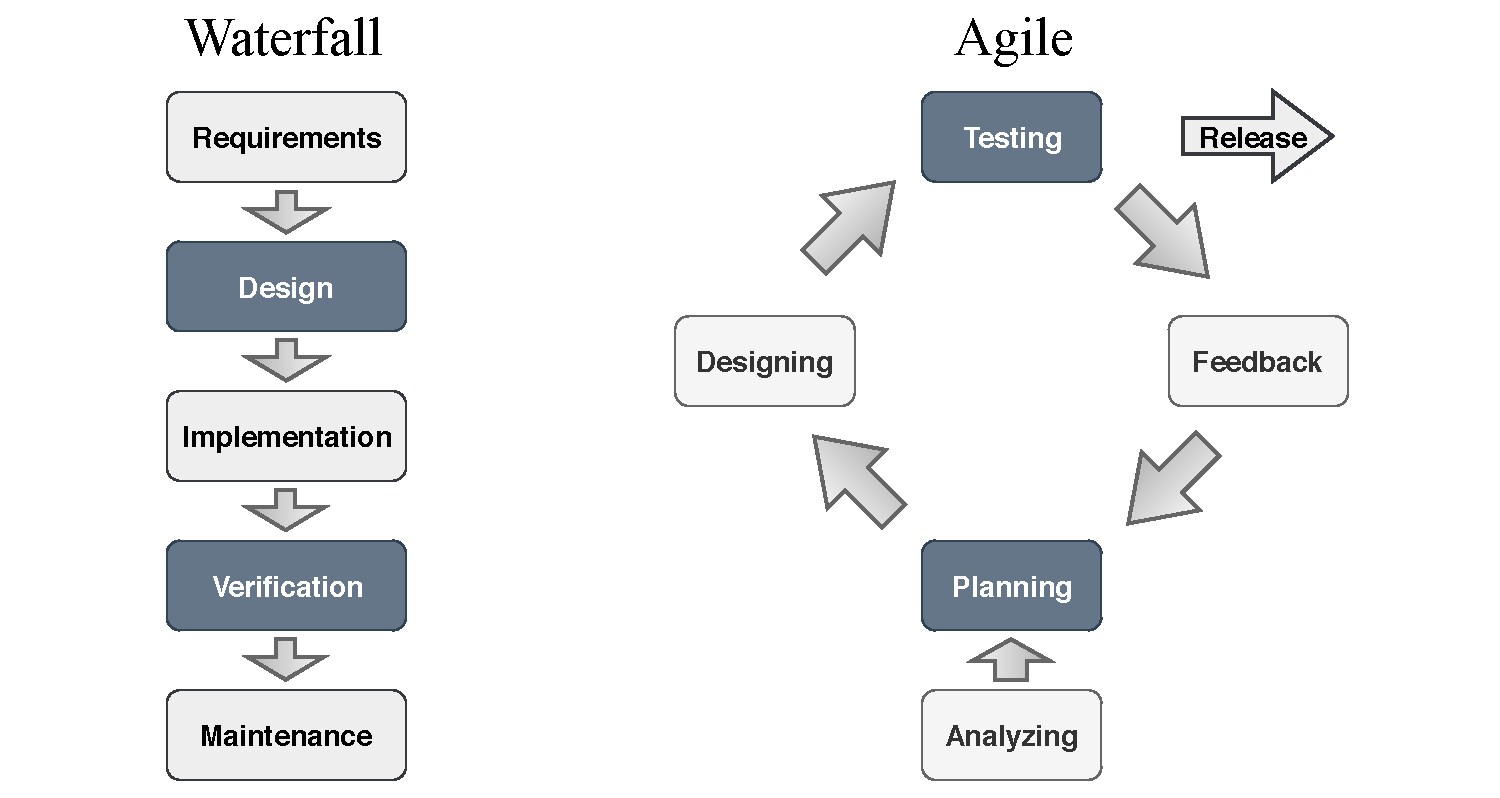
\includegraphics[width=0.5\textwidth]{water_grey.pdf}}
\caption{Waterfall vs. Agile in Software Development}    
\label{fig:water}
\end{figure}



Along with the changing of software development, more and more methods have been proposed and developed for software effort estimation. However,  one obvious trend is that people usually focus on developing and comparing new methods, but very few of them validated the performance of these state-of-the-art methods with classical models (e.g. COCOMO-II). As Menzies et al.~\cite{MenziesNeg:2017} mentioned, when dealing with COCOMO-Style effort datasets, COCOMO-II can still have the best estimates compared to other new methods. This fact tells us that any new software effort estimation methods should be analyzed and compared not only with state-of-the-art competitors, but also with old ones on formerly collected dataset. 


% It is necessary to develop new technique and make changes to improve traditional effort estimations. Robles et al. reports that more and more companies have started to turn their major interests to open source software projects (e.g. Agile software projects on GitHub), other than traditional waterfall style projects, for their new business strategy~\cite{robles2014estimating}. For old parametric estimating models like COCOMO, Shepperd et al. found it is difficult to determine some of their features for the estimations~\cite{shepperd2007software}. COCOMO measured software size by using LOC (line of code), but this feature is not available during the coding procedure, and it is difficult to make comparisons between different programming languages that may take varying numbers of statements to perform a given function. Jeffery et al. indicated that parametric model like COCOMO need to be calibrated to be used effectively in their study~\cite{jeffery1990calibrating}, which is another evidence that old parametric estimating models like COCOMO may not be appropriate for newer tasks. 

% As to the effort dataset, Peters et al. mentioned that the research of effort estimation traditionally suffers from severe shortage of effort data since these industrial data owners usually don't share their data to the public due to privacy concerns~\cite{peters2012privacy}. What's more, in real-world effort estimations, not only the size of data is limited, the variety of effort dataset is also incomplete since different industrial projects have different developing platform, characteristics or business related field, etc~\cite{qi2017software}.



% when trying to develop novel approach of software effort estimation tasks, we should also pay more attention on how are these new ones doing on old classical datasets.

% An important reason to keep finding new methods to replace COCOMO-Style models is that not all projects can be expressed in COCOMO. When COCOMO-Style datasets are available, Boehm's original procedure~\cite{boehm1981software} has valued performance result~\cite{MenziesNeg:2017}. When we want to extend our exploration beyond COCOMO domain, we do not have many choices but to find new methods that not only works on COCOMO-Style dataests, but also very recent ones.

Recently, many software researchers have demonstrated that hyperparameter tuning can dramatically improve software analytics tasks, like software defect prediction and text classification ~\cite{agrawal2017better,AGRAWAL2018,Fu2016TuningFS,tanti18,xia2018hyperparameter, fu2017easy}. The basic idea is that the default values of built-in parameters of those learning algorithms can not be the best fit for software analytics because of the naturalness of software engineering data~\cite{fu2016differential, hindle2012naturalness}. Therefore tuning the the control parameters of data
mining algorithms is becoming necessary for software anlaytics tasks~\cite{Fu2016TuningFS,tanti18}.


Based on the aforementioned two facts, we think that a new effort estimation baseline method should be based on parameter tuning methods and should be applicable to both COCOMO-style data and latest non-COCOMO software projects from Github. This paper proposed ``ROME'', a new effort estimation method, which is supercharged by fast hyperparameter optimization method. The applicability of this method has been verified  with the datasets both from classical Waterfall projects data (COCOMO), and novel open source Agile project data from GitHub. 


% The study is an extensive exploration  of
% hyperparameter optimization and effort estimation following the earlier work ~\cite{corazza2013using,xia2018hyperparameter}.

To assess our technique's effectiveness for effort estimation, as well as the compatibility for datasets from different source, this paper asks four research questions in our exploration. These questions have been selected based on our experience debating the merits of COCOMO vs alternate methods. We belive that each of the following questions can be used to motivate the development of some  novel estimation approachs:


{\bf \em RQ1: Does ``ROME'' have better performance than original COCOMO procedure?} The answer to this research question also answers the question thrown by Menzies et al.~\cite{MenziesNeg:2017}. 
We find that ``ROME'' provides, if not better, similar as COCOMO-II method, even in classical COCOMO-Style datasets. Hence, for effort estimation:
 \begin{result}{1}
 In the experiment with COCOMO-style datasets, ROME performs no worse than traditional COCOMO procedure.
 \end{result}

{\bf RQ2: \em  Can ``ROME'' achieve better results in non-COCOMO effort data?}
 This research question investigates the effectiveness our approach, to prove ROME not only works in COCOMO-style datasets, but also can help  do the effort estimation for recent projects can't be expressed in COCOMO-style. We observe that in data collected from open source projects on GitHub, our approach outperform other methods:
 \begin{result}{2}
 In the experiment with new datasets, ROME achieves superior performance compared to other methods.
 \end{result}
 
% {\bf RQ3:
%   \em Can hyperparameter tuning effort be saved by replacing  old defaults with new defaults?}
%  This  research question studies if we can run hyperparameter tuning once (and once only) then use those new defaults
%  ever after. From the experimental results, we find that optimal parameters of effort estimation differ dramatically
%  from dataset to dataset. Hence, for effort estimation:
%  \begin{result}{3}
%  Overall, there are no global ``best'' default settings and hyperparameter tuning should run for every project.
%  \end{result}

{\bf RQ3: \em When we have new effort datasets, what hyperparameter optimizers to use for effort estimation tasks?} Here, after combing the performance results from old and new datasets, we report that a certain combination  of learner and optimizer usually
produce best results:
\begin{result}{3}
For new datasets, try a combination of {\em CART} with the sequential model optimizer named {\em FLASH}.
\end{result}
% (Note: The {\it italicized} words are explained below.)


In summary, unlike the negative results found by Menzies et al.~\cite{MenziesNeg:2017}, for effort estimation tasks, our approach, ROME, achieves good performance results in both old COCOMO-Style datasets and non COCOMO newly collected open source datasets. Overall the contributions of this paper are:
\bi
\item Effort estimation based on hyperparameter tuning can achieve competitive performance in  decades-old COCOMO-style effort datasets. This helps to improve the compatibility for effort estimators. 

\item  Effort estimation based on hyperparameter tuning is useful for  effort estimation tasks where the project data can not be expressed in COCOMO-style because it provides superior performance in recent collected effort datasets on GitHub.

\item Defaults parameters of effort estimators are not the best fit for effort estimation. Hence, when new
data is encountered, some tuning process is required
to learn the best settings for generating estimates
from that data.

\item ``ROME'' as a new effort estimation framework works great on both COCOMO-style data and non COCOMO-style data should be considered as the next effort estimation baseline in this field.
% \item
% The identification of a  combination
% of learner and optimizer that  works
% as well as  any other effort estimation methods.
% \item An extensible open-source architecture called ROME that enables the commissioning of effort estimation methods.
% ROME makes our results   repeatable and refutable.
\ei
The rest of this paper is structured as follows.
The next section discusses the history and different methods for effort estimation tasks and how to optimize
the parameters of effort estimation methods. This is followed by a description of our experimental data, methods and the results. After that, a discussion section explores open issues with this work. 

From all of the above, we can conclude that (a)~ for effort estimation tasks, it is necessary to check if new approach works in old procedures and (b)~ hyperparamter tuning based approach is useful in both old COCOMO datasets and open source datasets.
Hence, we hope that ROME, and the results of  this paper,  will prompt and enable   more research on   methods
to develop software effort estimators.

Note that ROME and all the data used in this study is freely available for download from https://github.com/arennax/effort\_rome\_2019

\section{Background}
\label{sec:back}
Software effort estimation is the procedure to provide
approximate advice on how much human effort is required to plan, design and develop a software project. Usually, this human effort is expressed in terms of hours, days or months of human work. Since the nature of software, the development keeps being dynamic so the estimation can only be approximate. Still, doing estimation is necessary since it is important to allocate resources properly in software projects to avoid waste. In some cases, improper allocation of funding can cause a considerable waste of resource and time~\cite{cowing02,germano16,hazrati11,roman16}. 

Effort estimation in software development can be categorized into human-based and algorithm-based methods~\cite{teak2012,shepperd2007software}. In this paper we focus on algorithm-based methods since they are preferred when estimate have to be audited or debated (these methods is explicit and available for inspection). To understand the range of possible estimates, we can run the algorithm as many times as necessary, which may not be applicable by using human-based methods. Algorithm-based methods can have comparable performance to human-based ones. J{\o}rgensen et al. indicates that even very strong
advocates of human-based methods acknowledge that algorithm-based methods are useful for learning the uncertainty about particular estimates~\cite{jorgensen2009impact}.

Algorithm-based effort estimation methods have been widely explored in the past few decades. From very old classical model like COCOMO to recent proposed approach like ATLM~\cite{Whigham:2015} and LP4EE~\cite{SarroTOSEM2018}.

% It is known that humans rarely update their human-based estimation knowledge
% based on feedback from new projects~\cite{jorgensen2009impact}.

%  \begin{figure}[!t]
% {\scriptsize
% \begin{center}
% \begin{tabular}{|p{0.2in}|p{1.46in}|p{0.77in}|p{0.77in}|p{0.77in}|}\hline

%  & Definition & Low-end = \{1,2\}
%  &Medium =\{3,4\} &High-end= \{5,6\} \\\hline

% \multicolumn{1}{c}{~}\\

% \multicolumn{5}{l}{Scale factors:}\\\hline
% Flex   &  development flexibility   & development process
% rigorously defined & some guidelines, which can be relaxed & only
% general goals defined\\\hline

% Pmat    & process maturity  &  CMM level 1 &   CMM level 3  &  CMM level 5 \\\hline

% Prec & precedentedness  &  we have never built this kind
% of software before &    somewhat new &
% thoroughly familiar \\\hline

% Resl &  architecture or risk resolution  &  few interfaces
% defined or few risks eliminated  &  most interfaces defined or most
% risks eliminated   & all interfaces defined or all risks
% eliminated\\\hline

% Team  &   team cohesion  &  very difficult interactions &
% basically co-operative  &  seamless interactions\\\hline

% \multicolumn{1}{c}{~}\\

% \multicolumn{5}{l}{Effort multipliers}\\\hline
% acap  &  analyst capability  &  worst 35\% &   35\% - 90\% &  best 10\% \\\hline

% aexp   &  applications experience  &  2 months &   1 year  &  6 years\\\hline

% cplx   &  product complexity   & e.g. simple read/write
% statements & e.g. use of simple interface widgets  &  e.g.
% performance-critical embedded systems\\\hline

% data   &  database size 
% (DB bytes/SLOC) &
% 10 & 100 &    1000 \\\hline

% docu   &  documentation   & many life-cycle phases not
% documented      & &  extensive reporting for each life-cycle phase\\\hline

% ltex   &  language and tool-set experience   & 2 months  &  1
% year & 6 years \\\hline

% pcap   &  programmer capability  &  worst 15\%   & 55\%  &  best 10\% \\\hline

% pcon   &  personnel continuity \newline
% (\% turnover per year) &
%     48\% &    12\%  & 3\% \\\hline
% plex   &  platform experience  &  2 months  &  1 year  &  6 years\\\hline

% pvol   &  platform volatility ($\frac{frequency~of~major~changes}{frequency~of~minor~changes}$) &
% $\frac{12~months}{1~month}$   & $\frac{6~months}{2~weeks}$ &
% $\frac{2~weeks}{2~days}$\\\hline

% rely   &  required
% reliability &   errors are slight inconvenience  &  errors are easily
% recoverable   & errors can risk human life\\\hline

% ruse   &  required
% reuse &   none &    multiple program  & multiple product lines\\\hline

% sced  &   dictated development\newline schedule &    deadlines moved to
% 75\% of the original estimate &  no change
% &  deadlines moved back to  160\% of original estimate\\\hline

% site   &  multi-site development   & some contact: phone, mail&
% some email  &  interactive multi-media\\\hline

% stor  &   required \% of available
% RAM & N/A
%  &   50\% &  95\% \\\hline

% time  &   required \% of available CPU &
% N/A&     50\%
%   &  95\% \\\hline

% tool   &  use of software tools  &  edit,code,debug &&
% integrated with life cycle\\\hline

% \multicolumn{1}{c}{~}\\

% \multicolumn{5}{l}{Effort}\\\hline

% months & construction effort  in months& \multicolumn{3}{l|}{1 month =  152 hours (includes development \& management
% hours).  
% }\\\hline
% \end{tabular}
% \end{center}
% } \caption{COCOMO-II attributes.}
% \label{fig:cparems}
% \end{figure}


% \begin{table*}
% \caption{COCOMO-II attributes.}
% \label{tbl:cparems}
% \centerline{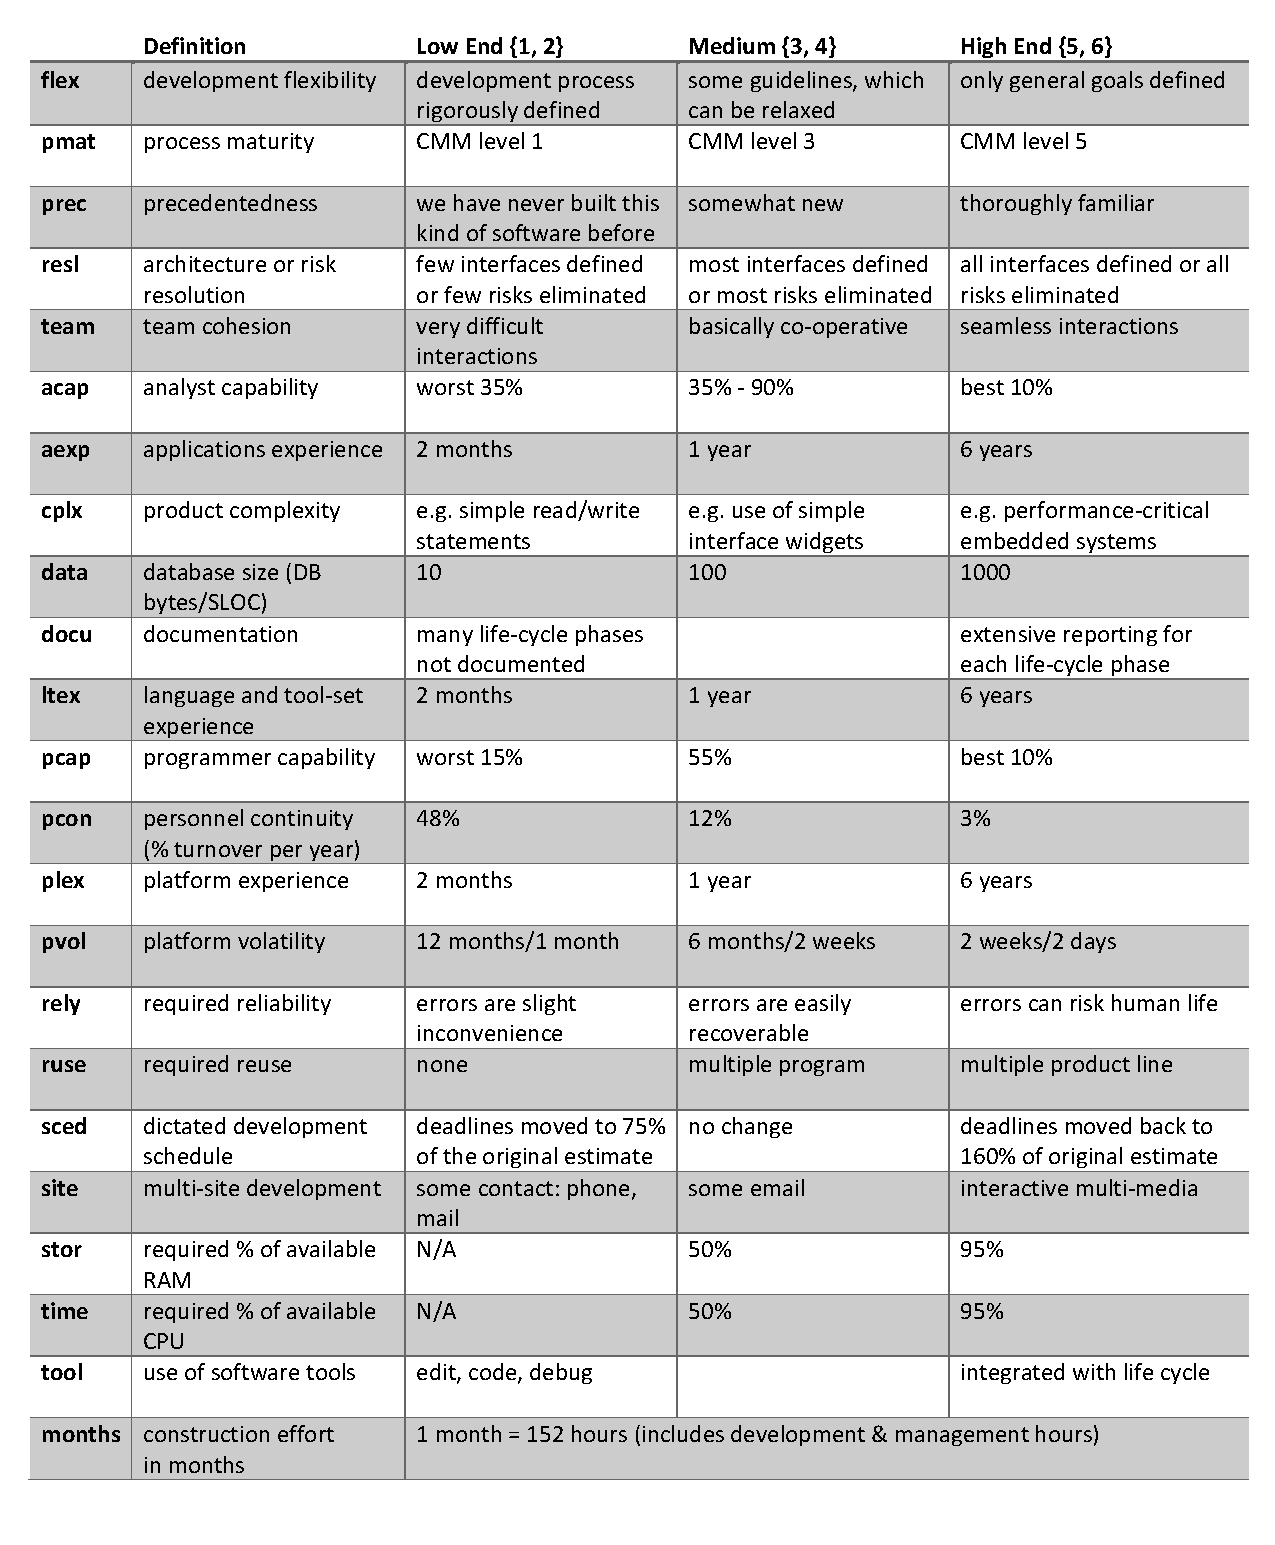
\includegraphics[width=.7\textwidth]{cocomo_para.pdf}}
% \end{table*}

\begin{table*}[!htbp]
\centering
\caption{COCOMO-II attributes.}
\begin{tabular}{c|l|l|l|l}
\hline
\rowcolor[HTML]{EFEFEF} 
 & \multicolumn{1}{c|}{\cellcolor[HTML]{EFEFEF}\textbf{Definition}} & \multicolumn{1}{c|}{\cellcolor[HTML]{EFEFEF}\textbf{Low End \{1, 2\}}} & \multicolumn{1}{c|}{\cellcolor[HTML]{EFEFEF}\textbf{Medium \{3, 4\}}} & \multicolumn{1}{c}{\cellcolor[HTML]{EFEFEF}\textbf{High End \{5, 6\}}} \\ \hline
\multicolumn{5}{l}{\textbf{Scale factors}} \\ \hline
flex & development flexibility & \begin{tabular}[c]{@{}l@{}}development process\\ rigorously defined\end{tabular} & \begin{tabular}[c]{@{}l@{}}some guidelines, which\\ can be relaxed\end{tabular} & only general goals defined \\ \hline
pmat & process maturity & CMM level 1 & CMM level 3 & CMM level 5 \\ \hline
prec & precedentedness & \begin{tabular}[c]{@{}l@{}}we have never built this \\ kind of software before\end{tabular} & somewhat new & thoroughly familiar \\ \hline
resl & architecture or risk resolution & \begin{tabular}[c]{@{}l@{}}few interfaces defined \\ or few risks eliminated\end{tabular} & \begin{tabular}[c]{@{}l@{}}most interfaces defined \\ or most risks eliminated\end{tabular} & \begin{tabular}[c]{@{}l@{}}all interfaces defined or all \\ risks eliminated\end{tabular} \\ \hline
team & team cohesion & very difficult interactions & basically co-operative & seamless interactions \\ \hline
\multicolumn{5}{l}{\textbf{Effort multipliers}} \\ \hline
acap & analyst capability & worst 35\% & 35\% - 90\% & best 10\% \\ \hline
aexp & applications experience & 2 months & 1 year & 6 years \\ \hline
cplx & product complexity & \begin{tabular}[c]{@{}l@{}}e.g. simple read/write\\ statements\end{tabular} & \begin{tabular}[c]{@{}l@{}}e.g. use of simple \\interface widgets\end{tabular} & \begin{tabular}[c]{@{}l@{}}e.g. performance-critical \\ embedded systems\end{tabular} \\ \hline
data & database size,(DB bytes/SLOC) & 10 & 100 & 1000 \\ \hline
docu & documentation & \begin{tabular}[c]{@{}l@{}}many life-cycle phases \\ not documented\end{tabular} &  & \begin{tabular}[c]{@{}l@{}}extensive reporting for \\each life-cycle phase\end{tabular} \\ \hline
ltex & language and tool-set experience & 2 months & 1 year & 6 years \\ \hline
pcap & programmer capability & worst 15\% & 55\% & best 10\% \\ \hline
pcon & \begin{tabular}[c]{@{}l@{}}personnel continuity \\ (\% turnover per year)\end{tabular} & 48\% & 12\% & 3\% \\ \hline
plex & platform experience & 2 months & 1 year & 6 years \\ \hline
pvol & \begin{tabular}[c]{@{}l@{}}platform volatility\\ ($\frac{frequency~of~major~changes}{frequency~of~minor~changes}$)\end{tabular} & $\frac{12~months}{1~month}$ & $\frac{6~months}{2~weeks}$ & $\frac{2~weeks}{2~days}$ \\ \hline
rely & required reliability & \begin{tabular}[c]{@{}l@{}}errors are slight \\ inconvenience\end{tabular} & \begin{tabular}[c]{@{}l@{}}errors are easily\\ recoverable\end{tabular} & errors can risk human life \\ \hline
ruse & required reuse & none & multiple program & multiple product lines \\ \hline
sced & dictated development schedule & \begin{tabular}[c]{@{}l@{}}deadlines moved to 75\% \\of the original estimate\end{tabular} & no change & \begin{tabular}[c]{@{}l@{}}deadlines moved back to, \\160\% of original estimate\end{tabular} \\ \hline
site & multi-site development & some contact: phone, mail & some email & interactive multi-media \\ \hline
stor & required\% of available RAM & N/A & 50\% & 95\% \\ \hline
time & required\% of available CPU & N/A & 50\% & 95\% \\ \hline
tool & use of software tools & edit, code, debug &  & integrated with life cycle \\ \hline
\multicolumn{5}{l}{\textbf{Effort}} \\ \hline
months & construction effort in months & \multicolumn{3}{c}{1 month = 152 hours (includes development \& management hours)} \\ \hline
\end{tabular}
\label{tbl:cparems}
\end{table*}

\subsection{COCOMO}
\label{sec:coco}

COCOMO (the COnstructive COst MOdel) is a procedural cost estimate model for software projects proposed by Boehm et al. based on LOC (number of Lines of Code). It is often used as a process of reliably predicting the various parameters associated with making a project such as size, effort, cost, time and quality. In late 1970s, Boehm was able to gather 63 project data points that could be published and to extend the model to
include alternative development modes that covered
other types of software such as business data
processing.  The resulting model was called the
Constructive Cost Model, or COCOMO, and was
published along with the data in the book Software
Engineering Economics~\cite{boehm1981software}. 
In this first version model (COCOMO-I), project attributes
were scored using just a few coarse-grained values (very low,
low, nominal, high, very high). These attributes
are {\em effort multipliers} where
a off-nominal value changes the estimate by some number
greater or smaller than one.
In COCOMO-I, all attributes (except KLOC)
influence effort in a linear manner.



% \begin{figure}[!t]
% \begin{center}
% \begin{lstlisting}
% _  = None;  Coc2tunings = [[
% #              vlow  low   nom   high  vhigh  xhigh   
% # scale factors:
% 'Flex',        5.07, 4.05, 3.04, 2.03, 1.01,    _],[
% 'Pmat',        7.80, 6.24, 4.68, 3.12, 1.56,    _],[
% 'Prec',        6.20, 4.96, 3.72, 2.48, 1.24,    _],[
% 'Resl',        7.07, 5.65, 4.24, 2.83, 1.41,    _],[
% 'Team',        5.48, 4.38, 3.29, 2.19, 1.01,    _],[
% # effort multipliers:        
% 'acap',        1.42, 1.19, 1.00, 0.85, 0.71,    _],[
% 'aexp',        1.22, 1.10, 1.00, 0.88, 0.81,    _],[
% 'cplx',        0.73, 0.87, 1.00, 1.17, 1.34, 1.74],[
% 'data',           _, 0.90, 1.00, 1.14, 1.28,    _],[
% 'docu',        0.81, 0.91, 1.00, 1.11, 1.23,    _],[
% 'ltex',        1.20, 1.09, 1.00, 0.91, 0.84,    _],[
% 'pcap',        1.34, 1.15, 1.00, 0.88, 0.76,    _],[ 
% 'pcon',        1.29, 1.12, 1.00, 0.90, 0.81,    _],[
% 'plex',        1.19, 1.09, 1.00, 0.91, 0.85,    _],[ 
% 'pvol',           _, 0.87, 1.00, 1.15, 1.30,    _],[
% 'rely',        0.82, 0.92, 1.00, 1.10, 1.26,    _],[
% 'ruse',           _, 0.95, 1.00, 1.07, 1.15, 1.24],[
% 'sced',        1.43, 1.14, 1.00, 1.00, 1.00,    _],[ 
% 'site',        1.22, 1.09, 1.00, 0.93, 0.86, 0.80],[ 
% 'stor',           _,    _, 1.00, 1.05, 1.17, 1.46],[
% 'time',           _,    _, 1.00, 1.11, 1.29, 1.63],[
% 'tool',        1.17, 1.09, 1.00, 0.90, 0.78,    _]]

% def COCOMO2(project,  a = 2.94, b = 0.91, # defaults
%                       tunes= Coc2tunings):# defaults 
%   sfs,ems,kloc   = 0, 5 ,22        
%   scaleFactors, effortMultipliers = 5, 17
  
%   for i in range(scaleFactors):
%     sfs += tunes[i][project[i]]
    
%   for i in range(effortMultipliers):
%     j = i + scaleFactors
%     ems *= tunes[j][project[j]] 
    
%   return a * ems * project[kloc] ** (b + 0.01*sfs) 
% \end{lstlisting}
% \end{center}
% \caption{COCOMO-II: effort estimates from a {\em project}.
% Here, {\em project} has  5 scale
% factors plus 17 effort multipliers plus KLOC. 
% ``Xhigh'' is show for ``extremely high''.
% Each attribute except KLOC and effort is scored
% using the scale very low = 1, low=2, up to
% xhigh=6.
% Note all attributes extend across the entire
% range very low to extremely high since,
% in Boehm's modeling work, not all effects extend
% across the entire range.
% For an explanation of the attributes shown in
% green, see \fig{cparems}.}\label{fig:coc2}
% \end{figure}


Boehm created a consortium for
industrial organizations after COCOMO was released.
It collected information on 161 projects from commercial,
aerospace, government, and non-profit organizations.
Based on an analysis of those 161 projects, new attributes called {\em scale factors} were added to the original model, which had an {\em exponential impact}
on effort.
Using the new data, Boehm et al. developed COCOMO-II model that map the project descriptors (very low, low, etc.)
into the specific values~\cite{boehm2000cost}:
% \begin{equation}\label{eq:cocII}
% \mathit{effort}=a\prod_i EM_i *\mathit{KLOC}^{b+0.01\sum_j SF_j}
% \end{equation}
\[
\mathit{effort}=a\prod_i EM_i *\mathit{KLOC}^{b+0.01\sum_j SF_j}
\]
Inside the function, $a,b$ are the {\em local calibration} parameters (with default values of 2.94 and 0.91). {\em EM} stands for effort multipliers, and {\em SF} are scale factors. The calculated {\em effort}
measures ``development months'' where one month is 152 hours of work  (and includes development and management hours). For details about COCOMO attributes, see \tbl{cparems}.

It is necessary to develop new technique and make changes to improve COCOMO. Robles et al. reports that more and more companies have started to turn their major interests to open source software projects (e.g. Agile software projects on GitHub), other than traditional waterfall style projects (e.g. COCOMO), for their new business strategy~\cite{robles2014estimating}. For old parametric estimating models like COCOMO, Shepperd et al. found it is difficult to determine some of their features for the estimations~\cite{shepperd2007software}. COCOMO measured software size by using LOC (line of code), but this feature is not available during the coding procedure, and it is difficult to make comparisons between different programming languages that may take varying numbers of statements to perform a given function. Jeffery et al. indicated that parametric model like COCOMO need to be calibrated to be used effectively in their study~\cite{jeffery1990calibrating}, which is another evidence that old parametric estimating models like COCOMO may not be appropriate for newer tasks. 

As to the effort dataset, there are very limited COCOMO dataset available for researchers. Peters et al. mentioned that the research of effort estimation traditionally suffers from severe shortage of effort data since these industrial data owners usually don't share their data to the public due to privacy concerns~\cite{peters2012privacy}. What's more, in real-world effort estimations, not only the size of data is limited, the variety of effort dataset is also incomplete since different industrial projects have different developing platform, characteristics or business related field, etc~\cite{qi2017software}.


\subsection{ATLM}
\label{sec:atlm}
Automatically Transformed Linear Model (ATLM) is a multiple linear regression model proposed by Whigham et al.~\cite{Whigham:2015}. It calculates the effort as:

\[
\mathit{effort} = \beta_0 + \sum_i\beta_i\times a_{i} +  \varepsilon_i
\]

where $a_i$ are explanatory attributes and $\varepsilon_i$ are errors to the actual value. The prediction weights $\beta_i$ are determined using least square error estimation~\cite{neter1996applied}. Additionally, transformations are applied on the attributes to further minimize the error in the model. In case of categorical attributes, the standard approach of ``dummy variables"~\cite{hardy1993regression} is applied. While, for continuous attributes, transformations such as logarithmic, square root,  or no transformation is employed such that the skewness of the attribute is minimum. 

It should be noted that, ATLM does not consider relatively complex techniques like using model residuals,  box transformations or step-wise regression (which are standard) when developing a linear regression model. The authors make this decision since they intend ATLM to be a simple baseline model rather than the ``best" model.


\subsection{LP4EE}
\label{sec:lp4ee}
Linear Programming for Effort Estimation (LP4EE) is a newly developed method by Sarro et al.~\cite{SarroTOSEM2018}, it aims to achieve the best outcome from a mathematical
model with a linear objective function subject to linear equality and inequality
constraints. The feasible region is given by the intersection of the constraints and the
Simplex (linear programming algorithm) is able to find a point in the polyhedron where
the function has the smallest error in polynomial time. In effort estimation problem, this model minimizes the Sum of Absolute Residual (SAR), when a new project is presented to the model, LP4EE predicts the effort as

\[
\mathit{effort} = a_1*x_1 + a_2*x_2 + ... + a_n*x_n
\]

where $x$ is the value of given project feature and $a$ is the corresponding coefficient evaluated by linear programming.
LP4EE is suggested to be used as another baseline model for effort estimation since it provides
similar or more accurate estimates than ATLM and is much less sensitive than ATLM
to multiple data splits and different cross-validation methods.

\subsection{Machine learning-based Effort Estimators}
\label{sec:algo}


% \begin{figure}
% \centerline{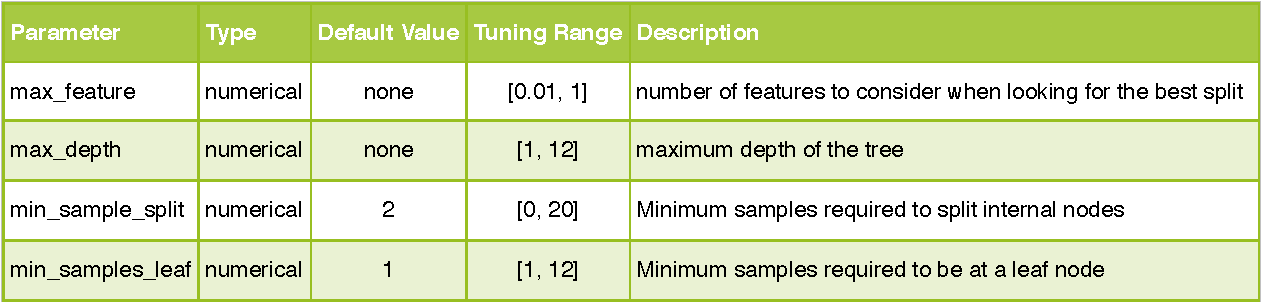
\includegraphics[width=1\textwidth]{table_cart.pdf}}
% \caption{CART's parameters.}\label{fig:cart}
% \end{figure}
\newcommand{\centered}[1]{\begin{tabular}{l} #1 \end{tabular}}



Typical machine learning algorithm are also used for software effort estimation. For example, Some algorithm-based estimators are regression trees such as CART~\cite{brieman84}, 
CART is a  tree learner that divides a dataset, then recurses
on each split.
If data contains more than {\em min\_sample\_split}, then a split is attempted.
On the other hand, if a split contains no more than {\em min\_samples\_leaf}, then the recursion stops. 
CART finds the attributes whose ranges contain rows with least variance in the number
of defects. If an  attribute ranges $r_i$ is found in 
$n_i$ rows each with an effort  variance of $v_i$, then CART seeks the  attribute with a split that most
minimizes $\sum_i \left(\sqrt{v_i}\times n_i/(\sum_i n_i)\right)$.
For more details on the CART parameters, see Table~\ref{tbl:cart}.

% \begin{table*}[!t]
% \centering
% \caption{CART's parameters.}
% \begin{tabular}{l|c|c|c|p{1.6in}}
% \hline \rowcolor{black!30}
% Parameter  &Type        & Default & Tuning Range  & Description     \\\hline
% max\_feature & numerical      & None    & {[}0.01, 1{]} &Number of features to consider when looking for the best spilt. \\
% \rowcolor{black!15} max\_depth  &numerical       & None    & {[}1, 12{]}   & The maximum depth of the decision tree.                                     \\
% min\_sample\_split & numerical & 2       & {[}0, 20{]}   & Minimum   samples required to split  internal nodes.  \\
% \rowcolor{black!15} min\_samples\_leaf & numerical& 1       & {[}1, 12{]}   &   Minimum   samples required to be at a leaf node.    \\\hline
% \end{tabular}
% \end{table*}

\begin{table*}[!htbp]
\centering
\caption{CART's parameters.}
\begin{tabular}{l|c|c|c|l}
\hline
\rowcolor[HTML]{EFEFEF} 
\multicolumn{1}{c|}{\cellcolor[HTML]{EFEFEF}\textbf{Parameter}} & \textbf{Type} & \textbf{Default} & \textbf{Tuning Range} & \multicolumn{1}{c}{\cellcolor[HTML]{EFEFEF}\textbf{Description}} \\ \hline
max\_feature & numerical & None & {[}0.01, 1{]} & \begin{tabular}[c]{@{}l@{}}Number of features to consider\\ when looking for the best split\end{tabular} \\ \hline
max\_depth & numerical & None & {[}1, 12{]} & \begin{tabular}[c]{@{}l@{}}The maximum depth of the\\ decision tree\end{tabular} \\ \hline
min\_sample\_split & numerical & 2 & {[}0, 20{]} & \begin{tabular}[c]{@{}l@{}}Minimum samples required to \\ split internal nodes\end{tabular} \\ \hline
min\_sample\_leaf & numerical & 1 & {[}1, 12{]} & \begin{tabular}[c]{@{}l@{}}Minimum samples required to\\ be at a leaf node\end{tabular} \\ \hline
\end{tabular}
\label{tbl:cart}
\end{table*}




Random Forest~\cite{breiman2001random} and Support Vector Regression~\cite{chang2011libsvm} are another instances of regression methods. Random Forest (RF) is an ensemble learning method for  regression (and classification) tasks that  builds a set of   trees when training the model. To decide the output, it uses 
the mode of the classes (classification) or mean prediction (regression) of the individual trees.
Support Vector Regression (SVR) uses kernel functions to project
the data onto a new hyperspace where complex non-linear patterns
can be simply represented. It aims to construct an optimal hyperplane that fits data and predicts with
minimal empirical risk and complexity of the modelling function.

Another algorithm-based estimators are the 
Analogy-based Estimation (ABE) methods advocated by Shepperd and Schofield~\cite{shepperd1997estimating}. ABE is widely-used~\cite{7194627,Kocaguneli2015,7426628,6092574,MenziesNeg:2017}, in many forms.
We  say that  ``ABE0'' is the standard  form  seen in the literature
and ``ABEN'' are the 6,000+ variants of ABE  defined below. 
The general form of ABE (which applies to  ABE0 or ABEN) is
to first form a table of rows of past projects. The {\em columns} of this table are composed of independent variables (the {\em features} that define projects) and one dependent {\em feature} (project  effort).
From this table, we learn  what  similar projects (analogies) to use from the training set when examining a new test instance.
For each test instance, ABE then selects   $k$ analogies out of the training set.
Analogies are selected via   a {\em similarity measure}. 
Before calculating similarity,  ABE normalizes   numerics  min..max to 0..1 (so all numerics   get equal chance to influence the dependent). 
Then, ABE uses {\em feature} weighting to reduce the influence of less informative {\em features}.
Finally, some  {\em adaption strategy} is applied  return a combination of  the dependent effort values seen in  the $k$ nearest analogies. 

\subsection{Hyperparameter Optimization} \label{sec:tuning}


% \begin{figure}
% \vspace{0.5cm}
% \centerline{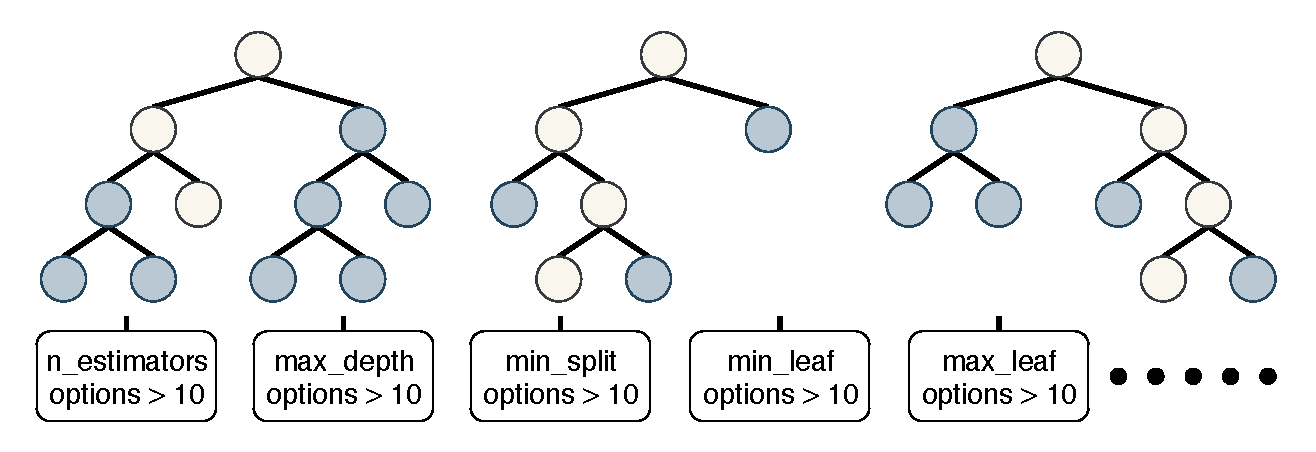
\includegraphics[width=1\textwidth]{randomforest_grey.pdf}}
% \caption{Hyperparameter options for a machine learning algorithm, Random Forest.  Only five hyperparameters are shown in the figure due to the space limitation. Note that all of them have more than 10 options.}    
% \label{fig:rfoptions}
% \end{figure}


Hyperparameters are the parameters that can require different constraints, weights or learning rates to generate different data patterns in machine learning models. Unlike the other parameters, the value of hyperparameter is set before the learning process begins, rather than derived via training process. These hyperparameters are important since they control the behaviors of the training algorithm and impact the performance of the model being trained directly. Therefore, choosing appropriate hyperparameters plays a critical role in the performance of machine learning models. Tuning hyperparameter is the process of searching the most optimal hyperparameter options for machine learning models~\cite{biedenkapp2018hyperparameter,franceschi2017forward}.
Some popular methods to tune the hyperparameters are grid search, random search and differential evolution.


\textit{Grid search}~\cite{bergstra2011algorithms} is a technique that using brute force of all combinations for hyperparameters. Although the Grid search method is a simple algorithm to use, it suffers if data have high dimensional space called the ``curse of dimensionality’‘. Previous work has shown that grid search might also miss important optimization~\cite{fu2016differential} and is a time-wasting process since only a few of the tuning parameters really matters~\cite{Bergstra:2012}.


\textit{Random search}~\cite{Bergstra:2012} randomly samples the search space and evaluates sets from a specified probability distribution. The drawback of using random search algorithm is that it does not use information from prior experiment to select the next set and also it is very difficult to predict the next of experiments.

\textit{Differential evolution} (DE)~\cite{storn1997differential} optimizes a problem by maintaining a population of candidate solutions and creating new candidate solutions by combining existing ones according to its simple formulae, and then keeping whichever candidate solution has the best score or fitness on the optimization problem. One thing to note is that DE does not guarantee an optimal solution is ever found.


\textit{Bayesian optimization}~\cite{pelikan1999simple} works by assuming the unknown function was sampled from a Gaussian Process and maintains a posterior distribution for this function as observation are made. However, it might not be well-suited for optimization over continuous domains with large number of dimensions~\cite{frazier2018tutorial}.

Hyperparameter optimization can be a tedious and time consuming task~\cite{fu2016differential}. 
% For example, consider, an effort estimator introduced above in above section, as shown in \fig{rfoptions}, Random Forest has more than
% $10^5 = 100,000$ different combinations depending on its hyperparameters. Similarly, 
For example, estimator ``ABEN'' has 6,000+ variants. Given the space to exploration is so large for these estimators, Trying all possible solutions may not be practical these tasks. Recently we've learned how to do it with just a few dozen samples as apposed to the thousands to millions of samples needed for traditional methods like grid searchers.
In this paper, we apply ROME architecture for exploring hyperparameter optimization and effort estimation. ROME uses the state-of-the-art optimizer (FLASH~\cite{nair2017flash}) to tune regression estimator CART~\cite{brieman84}, for software effort estimation tasks. 

\begin{figure}
\centerline{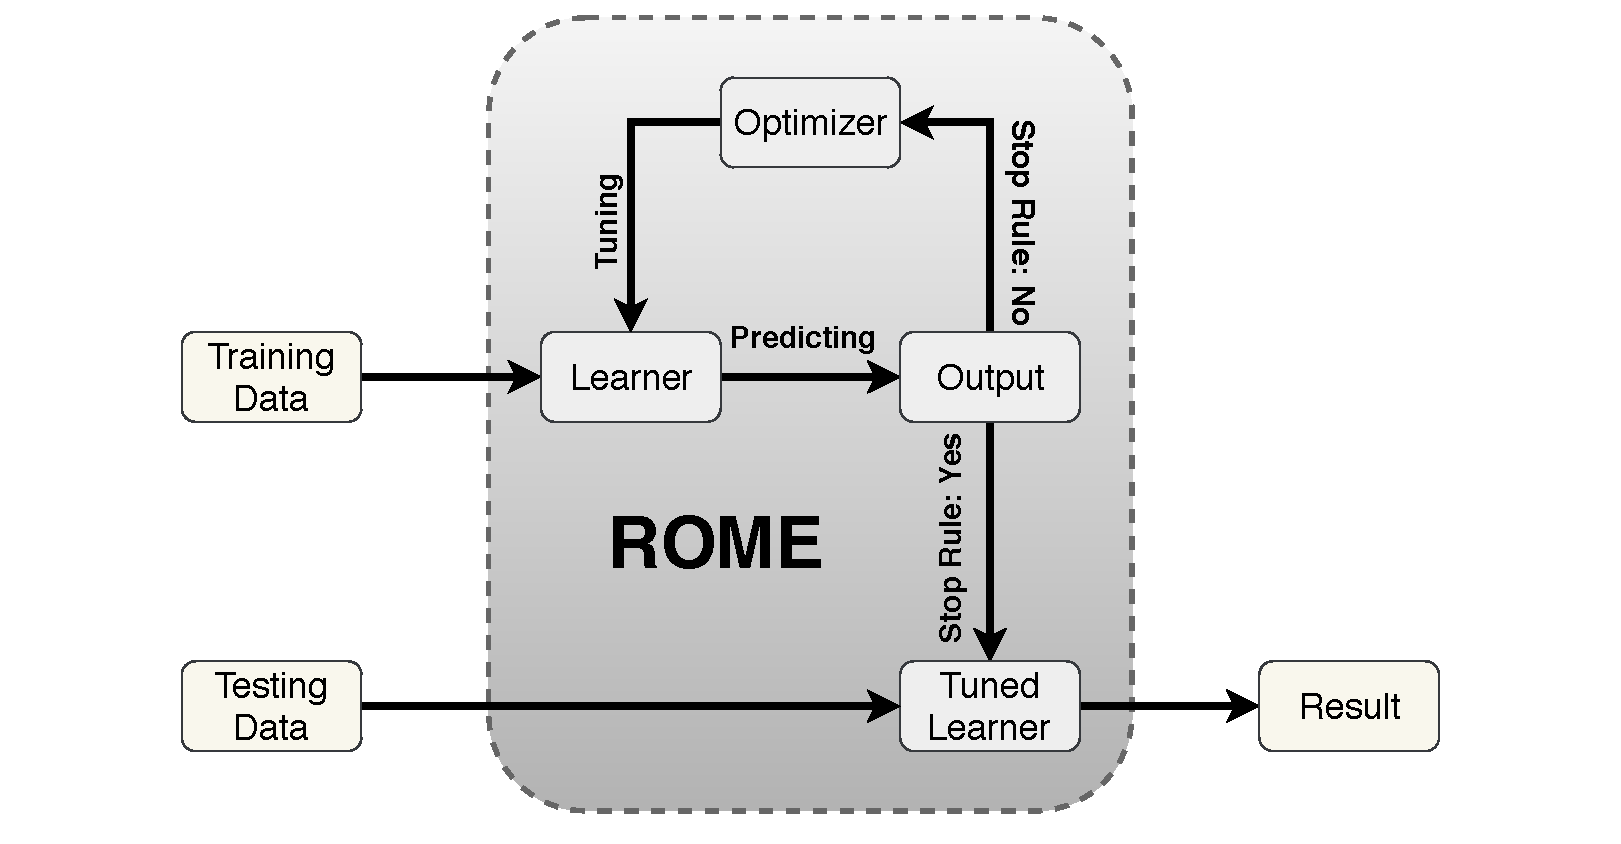
\includegraphics[width=0.55\textwidth]{rome_grey.pdf}}
\caption{ROME's architecture}    
\label{fig:romearc}
\end{figure}



\section{Method}
\label{sec:optim}
In this section, we firstly have an overview of the ROME framework, and then present each component in details. The architecture of ROME is shown in \fig{romearc}. ROME is a refined version of OIL, a configurable effort estimating technique introduced by Xia et al.~\cite{xia2018hyperparameter}.






Inside the ROME's architecture, we have a learning layer and a optimizing layer. When training data arrive, the estimator in the learning layer is being trained, and the optimizer in optimizing layer helps to improve the performace of estimators, until the stopping criteria is reached. Then the optimized estimator executes prediction on testing data.

It was simple  to ``pop the top'' and replace the optimizing layer with another optimizer. In this layer, ROME used FLASH~\cite{nair2017flash} as the optimizer.

\begin{figure}
\begin{pythoncode}
    # Pick a number of data into build_pool, 
    # evaluate the build_pool, 
    # and put the rest into rest_pool
    while life > 0:
      build CART model by using build_pool
      next_point = max(model.predict(rest_pool))
      build_pool += next_point
      rest_pool -= next_point
      if model.evaluate(next_point) < max(build_pool):
          life -= 1
    return max(build_pool)
\end{pythoncode}
\caption{Pseudocode of FLASH.}\label{flash}  
\end{figure}



FLASH, proposed by Nair et al.~\cite{nair2017flash}, is an incremental optimizer.
Previously, it has been applied to configuration system parameters for software systems. But for effort estimation, FLASH has not been extensively explored.
Formally, FLASH is a   {\em sequential model-Based optimizer}~\cite{bergstra2011algorithms} (also known
in the machine learning literature
as an {\em active learner}~\cite{das16} or, in  the statistics literature  as 
{\em optimal experimental design}~\cite{olsson2009literature}). No matter whatever the name is, the idea behind it is the same:
reflects on the model built to date in order to find the next best example
to evaluate. To tune a learning algorithm, FLASH explores $N$ possible tunings as follows:
\begin{enumerate}
\item
Set the evaluation budget $b$. In order to make a fair comparison between FLASH and other methods, we used $b=200$.
 \item
Run the learning algorithm with $n=20$ to randomly select tunings.
\item Build an {\em archive} of  $n$   examples holding pairs of  parameter settings and   their resulting performance scores
(e.g. MRE, SA, etc).
\item
Using that archive, learn a {\em surrogate}   to predicts performance. 
Following the methods of Nair et al.~\cite{nair2017flash}, we used   CART~\cite{brieman84}
for that surrogate.
\item Use the surrogate to guess  $M$ performance scores where
$M<N$ and $M \gg n$ parameter settings. Note that this step is very fast because all required is to run $M$ vectors downards some very small CART trees.
\item Using some {\em selection  function} to select  the most ``interesting'' setting. According to Nair et al.~\cite{nair2017flash} 
we returned the setting with the nearest prediction (i.e. find the most promising possibility).
\item Collect performance scores by evaluating    ``interesting'' using
the data miners (i.e. check the most troubling
possibility). Set $b=b-1$.
\item  Add  ``interesting'' to the archive. If  $b>0$, goto step 4. Else, halt.
\end{enumerate}



% We compare the performance of FLASH with Differential Evolution (hereafter, DE~\cite{storn1997differential}). The premise of DE is that the best way to mutate the existing tunings is to extrapolate between current solutions. Three solutions $a, b, c$ are selected at random. For each tuning parameter $k$, at some probability $cr$, we replace the old tuning $x_k$ with $y_k$. For
% booleans $y_k = \neg x_k$ and for numerics, 
% \mbox{$y_k = a_k + f \times (b_k - c_k)$}
% where $f$ is a parameter controlling differential weight.  
% The main loop of DE runs over the population of size $np$, replacing old items with new candidates (if new candidate is better). This means that, as the loop progresses, the population is full of increasingly more valuable solutions (which, in turn,
% helps   extrapolation). 
% As to the control parameters of DE,  using advice from Storn and Fu et al.~\cite{storn1997differential,Fu2016TuningFS}, we set $\{\mathit{np,g,cr}\}=\{20,0.75,0.3\}$. Also,
% the number of generations $\mathit{gen}$ was set to 10 to test
% the effects of  a very   CPU-light    effort estimator. 


In summary,  given what we already know about the tunings (represented in a CART tree),
FLASH finds the potentially best tunings (in Step 6); then evaluate the performance~(in Step 7); 
then  updates the model with the results of that evaluation.



\section{Empirical Study} \label{sect:study} 
\subsection{Research Questions}
To systematically evaluate ROME framework as a new baseline for effort estimation,  we asked the following research questions:
\bi
\item RQ1: Does ROME have better performance than original COCOMO procedure?
\item RQ2: Can ROME achieve better results in non-COCOMO effort data?
% \item  RQ3: Can hyperparameter tuning effort be saved by replacing  old defaults with new defaults?
\item RQ3: When we have new effort datasets, what hyperparameter optimizers to use for effort estimation tasks?
\ei
RQ1 and RQ2 is to investigate how ROME performs compared with other methods on COCOMO-sytle data and non COCOMO-style data. Since hyperparameter tuning has a great impact on the performance of the estiamtors, RQ3 lead us to study how hyperparameter tuning should be conducted in the effort estimation. 


\subsection{Dataset and Experimental Design}

\begin{table*}[!t]
\caption{\textcolor{black}{ The example of NASA10 dataset (one row per project). For a definition of the terms in row1 (``prec'', ``flex'', ``resl'' etc.) see \tbl{cparems}.
As to the different columns, scale factors change effort exponentially while effort multipliers have a linear impact on effort.
Any effort multiplier with a value of ``3'' is a {\em nominal} value; i.e. it multiplies the effort by a multiple of 1.0. Effort multipliers
above and below ``3'' can each effect project effort by a multiple ranging from 0.7 to 1.74.  
% For full details on how these values are used, see \fig{coc2}.
}}\label{tbl:nasa10}
    
  \small
  \setlength{\tabcolsep}{2.5pt}
\begin{tabu}{|ccccc|ccccccccccccccccc|c|c|}\hline
\rowfont{\color{white}} \rowcolor{black!70} prec&flex&resl&team&pmat&rely&cplx&data&ruse&     time&stor&pvol&acap&pcap&pcon&aexp&plex&     ltex&tool&sced&site&docu&kloc&months\\\hline
2&2&2&3&3&4&5&4&3&5&6&4&4&4&3&4&3&3&1&3&4&4&77&1830\\
\rowcolor{black!20}2&2&2&3&3&5&5&2&3&5&6&2&4&3&3&2&1&2&2&3&4&4&24&648\\
2&2&2&3&3&4&5&3&3&5&5&4&3&3&3&3&2&2&1&3&4&4&23&492\\
\rowcolor{black!20}2&2&3&3&2&4&4&3&2&3&3&4&3&3&3&3&3&4&2&3&5&3&146&3292\\
2&3&3&5&3&3&4&3&2&4&4&2&5&5&4&5&1&5&3&3&6&3&113&1080\\\hline
% 3&3&3&3&3&3&4&3&2&3&3&3&3&3&3&4&3&4&2&3&4&3&184&1043\\
% 5&3&3&3&4&4&4&3&2&3&3&2&3&3&3&5&3&4&2&3&5&3&61&336\\
% 5&3&3&4&4&4&5&3&2&3&3&2&3&3&3&5&3&4&2&3&6&3&50&637\\
% 3&3&3&2&3&4&5&3&2&3&3&3&3&3&3&4&3&4&2&3&5&3&253&2519\\
% 3&3&4&3&3&4&4&3&4&3&3&2&3&4&3&3&1&4&5&3&2&3&159&1048\\
% 3&3&3&3&3&4&5&3&2&3&3&4&4&4&5&4&4&4&2&1&5&3&324&1735\\
% 3&2&4&4&3&4&5&3&4&3&4&5&4&4&3&4&4&3&4&2&6&3&224&691\\
% 5&2&2&4&3&4&3&3&4&5&4&3&4&4&3&4&4&4&3&3&3&3&105&320\\
% 3&2&2&4&3&4&3&3&3&3&3&2&4&4&3&4&4&4&3&3&3&3&173&329\\
% 3&2&4&3&3&4&5&3&4&3&3&4&3&4&4&4&3&3&3&3&5&3&597&1705\\
% 4&2&4&3&5&4&3&2&3&3&4&4&2&2&3&3&5&5&3&3&5&3&155&789\\
% 4&3&3&3&4&4&4&3&2&3&3&3&4&4&3&5&4&4&2&3&5&3&170&552\\\hline 
\noalign{\vspace{-7pt}}
\multicolumn{5}{c}{$\underbrace{\hspace*{28\tabcolsep}}$}&
\multicolumn{17}{c}{$\underbrace{\hspace*{120\tabcolsep}}$}&
\multicolumn{1}{c}{$\underbrace{\hspace*{5\tabcolsep}}$} &
\multicolumn{1}{c}{$\underbrace{\hspace*{5\tabcolsep}}$}\\
\multicolumn{5}{c}{\bf \normalsize scale factors} & \multicolumn{17}{c}{\bf \normalsize effort multipliers} & \multicolumn{1}{c}{\bf \normalsize size} & \multicolumn{1}{c}{\bf \normalsize effort}\\
\end{tabu}
\end{table*}



To evaluate the proposed ROME framework comprehensively, we include COCOMO-style data and non COCOMO-style data. For COCOMO-style data, we include 216 projects from the SEACRAFT repository\footnote{http://tiny.cc/seacraft}; In \tbl{nasa10}, we list a sample of our data. This dataset has been widely used to evaluate effort estimation methods for COCOMO-sytle data, which serves the same purpose to compare our proposed framework with the COCOMO-II procedure. 
To test how ROME perform on non COCOMO data, we use data  collected from  446 projects on Github by Qi et al.~\cite{qi2017software} from Github. 
%In Qi et al.'s work, they implemented a platform for GitHub data crawling and filtering, and extracting necessary information for effort estimation tasks. They also propose a specific algorithm to make the collected dataset have dynamic expansion capability~\cite{qi2017software}. Using the datasets from Qi et al., we can validate our approach's effectiveness in recent software effort estimating tasks. % 
According to Qi et al.~\cite{qi2017software}, they define 7 features: EI, EO, LOC, AFP, APEX, LPEX, FILES. We list all statistics about this dataset and the descriptions about these features in Table~\ref{table:dataset}. 

Note that some features of the original Qi et al.'s datasets are not used in our experiment because they are (1) irrelevant to the effort values (e.g., ID), (2) unavailable at the prediction phase (e.g., LOC). A data cleaning process is applied to solve this issue. 
Those removed features are highlighted as italic in Table~\ref{table:dataset}.





\newcommand{\IT}[1]{\textcolor{red}{{\em #1}}}
\pdfoutput=1
\begin{table*}[t!]
\caption{Descriptive Statistics of the Datasets. EI and EO are the elementary process that processes data or control information sent from/to outside the boundary. Files are user recognizable groups of logically related data or control information maintained within the boundary, APEX and LPEX are Application and Language/Tool experience. AFP and LOC are Automated function point and Line of code. Terms in \IT{red} are removed from this study, for reasons discussed in the text.}\label{table:dataset}

\renewcommand{\baselinestretch}{0.75} 
\resizebox{.8\textwidth}{!}{
\centering
\begin{tabular}{cc}
\scriptsize
\begin{tabular}{|c|l|rrrr|}
    \hline
      & feature & min  & max & mean & std\\
  \hline
%%%%%%%%%%%%%%%%%%%%%%%%%%%%%%%%%%%%%%%%%%%%%%%%%%%%%%%%%%%%%%%%%%%%

\multirow{7}{*}{\begin{sideways}java\_init\end{sideways}}
& \IT{LOC} & 5 & 31 & 14.3 & 7.5\\
& EI & 39 & 450 & 186.6 & 136.8\\
& EO & 100 & 2307 & 999.1 & 589.6\\
& AFP & 97 & 2284 & 993.9 & 597.4\\
& APEX & 39 & 450 & 186.6 & 136.8\\
& LPEX & 100 & 2307 & 999.1 & 589.6\\
& FILES & 97 & 2284 & 993.9 & 597.4\\
& Effort & 23 & 1107 & 219.2 & 263.1\\
\hline
\multirow{7}{*}{\begin{sideways}java\_incre\end{sideways}}
& \IT{LOC} & 5 & 31 & 14.3 & 7.5\\
& EI & 39 & 450 & 186.6 & 136.8\\
& EO & 100 & 2307 & 999.1 & 589.6\\
& AFP & 97 & 2284 & 993.9 & 597.4\\
& APEX & 39 & 450 & 186.6 & 136.8\\
& LPEX & 100 & 2307 & 999.1 & 589.6\\
& FILES & 97 & 2284 & 993.9 & 597.4\\
& Effort & 23 & 1107 & 219.2 & 263.1\\
\hline
\multirow{7}{*}{\begin{sideways}java\_final\end{sideways}}
& \IT{LOC} & 5 & 31 & 14.3 & 7.5\\
& EI & 39 & 450 & 186.6 & 136.8\\
& EO & 100 & 2307 & 999.1 & 589.6\\
& AFP & 97 & 2284 & 993.9 & 597.4\\
& APEX & 39 & 450 & 186.6 & 136.8\\
& LPEX & 100 & 2307 & 999.1 & 589.6\\
& FILES & 97 & 2284 & 993.9 & 597.4\\
& Effort & 23 & 1107 & 219.2 & 263.1\\
\hline
\end{tabular} 
%%%%%%%%%%%%%%%%%%%%%%%%%%%%%%%%%%%%%%%%%%%%%%%%%%%%%%%%%%%%%%%%%%%%


~

\scriptsize
\begin{tabular}{|c|l|rrrr|}
    \hline
      & feature
    & min  & max & mean & std\\
  \hline
\multirow{7}{*}{\begin{sideways}webshop\_init\end{sideways}}
& \IT{LOC} & 5 & 31 & 14.3 & 7.5\\
& EI & 39 & 450 & 186.6 & 136.8\\
& EO & 100 & 2307 & 999.1 & 589.6\\
& AFP & 97 & 2284 & 993.9 & 597.4\\
& APEX & 39 & 450 & 186.6 & 136.8\\
& LPEX & 100 & 2307 & 999.1 & 589.6\\
& FILES & 97 & 2284 & 993.9 & 597.4\\
& Effort & 23 & 1107 & 219.2 & 263.1\\
\hline
\multirow{7}{*}{\begin{sideways}webshop\_incre\end{sideways}}
& \IT{LOC} & 5 & 31 & 14.3 & 7.5\\
& EI & 39 & 450 & 186.6 & 136.8\\
& EO & 100 & 2307 & 999.1 & 589.6\\
& AFP & 97 & 2284 & 993.9 & 597.4\\
& APEX & 39 & 450 & 186.6 & 136.8\\
& LPEX & 100 & 2307 & 999.1 & 589.6\\
& FILES & 97 & 2284 & 993.9 & 597.4\\
& Effort & 23 & 1107 & 219.2 & 263.1\\
\hline
\multirow{7}{*}{\begin{sideways}webshop\_final\end{sideways}}
& \IT{LOC} & 5 & 31 & 14.3 & 7.5\\
& EI & 39 & 450 & 186.6 & 136.8\\
& EO & 100 & 2307 & 999.1 & 589.6\\
& AFP & 97 & 2284 & 993.9 & 597.4\\
& APEX & 39 & 450 & 186.6 & 136.8\\
& LPEX & 100 & 2307 & 999.1 & 589.6\\
& FILES & 97 & 2284 & 993.9 & 597.4\\
& Effort & 23 & 1107 & 219.2 & 263.1\\
\hline
\end{tabular} 
\end{tabular}
}
\end{table*}


In the experiment, we use a {\em M*N-way} cross-validation to split training and testing data for the estimators. That is, in $M$ times,  shuffle the data randomly (using a different random number seed)
then divide the data into $N$ bins.
For $i   \in N$, bin $i$ is used to test a model
build from the other bins.
Following the advice
of Nair et al.~\cite{nair18}, we  use $N=3$  and $M=20$
for our effort datasets.   

As a procedural detail, first we divided the data and then we applied the treatments. That is, all treatments saw the same training and test data.

% \subsection{Terminology for Optimizers}

% Some treatments are named ``X\_Y'' which  denote learner ``X'' tuned by optimizer ``Y''.
% In the following: 

% {\small \begin{eqnarray} 
% X &\in &\{\mathit{CART}\}\nonumber\\
% Y &\in &\{\mathit{DE},\mathit{FLASH}\}\nonumber
% \end{eqnarray}}


In this experiment,  we do not tune COCOMO\_II, ATLM and LP4EE since they were designed to be used ``off-the-shelf''.  Whigham et al.~\cite{Whigham:2015} declare that one of ATLM's most important features is that if does not need tuning.
We also do not tune SVR and RF since we treat them as baseline algorithm-based methods in our benchmarks (i.e. use default settings in scikit-learn for these algorithms). Here, we add ABE0 and CART0 (CART with default settings) to compare the performance as well.

We compare the performance of our optimizer FLASH with Differential Evolution. The premise of DE is that the best way to mutate the existing tunings is to extrapolate between current solutions. Three solutions $a, b, c$ are selected at random. For each tuning parameter $k$, at some probability $cr$, we replace the old tuning $x_k$ with $y_k$. For
booleans $y_k = \neg x_k$ and for numerics, 
\mbox{$y_k = a_k + f \times (b_k - c_k)$}
where $f$ is a parameter controlling differential weight.  
The main loop of DE runs over the population of size $np$, replacing old items with new candidates (if new candidate is better). This means that, as the loop progresses, the population is full of increasingly more valuable solutions (which, in turn,
helps   extrapolation). 
As to the control parameters of DE,  using advice from Storn and Fu et al.~\cite{storn1997differential,Fu2016TuningFS}, we set $\{\mathit{np,g,cr}\}=\{20,0.75,0.3\}$. Also,
the number of generations $\mathit{gen}$ was set to 10 to ensure DE have same number of total explorations as FLASH.


\subsection{Performance Metrics}



The results from each test set are evaluated in terms of two scoring metrics:  magnitude of the relative error (MRE) and Standardized Accuracy (SA). 

MRE is defined in terms of 
AR,  the magnitude of the absolute residual. This is  computed from the difference between predicted and actual effort values:
\[
\mathit{AR} = |\mathit{actual}_i - \mathit{predicted}_i|
\] 
MRE is the magnitude of the relative error calculated by expressing AR as a ratio of   actual effort:
\[
\mathit{MRE} = \frac{|\mathit{actual}_i - \mathit{predicted}_i|}{\mathit{actual}_i}
\]

MRE is criticized by some researchers as it is biased towards error underestimations~\cite{foss2003simulation,kitchenham2001accuracy,korte2008confidence,port2008comparative,shepperd2000building,stensrud2003further}. Nevertheless, we use it here
since  there exists known baselines for human performance in effort estimation expressed in terms of MRE~\cite{Jorgensen03}. 
 
Because of the issues with MRE, some researchers prefer the 
use of other (more standardized) measures, such as  Standardized Accuracy (SA)~\cite{langdon2016exact,shepperd2012evaluating}.
SA is based on Mean Absolute Error (MAE), which is defined in terms of 
\[
\mathit{MAE}=\frac{1}{N}\sum_{i=1}^n|\mathit{RealEffort}_i-\mathit{EstimatedEffort}_i|
\]
where $N$ is the number of projects used for evaluating the performance, SA uses MAE as follows:
\[
\mathit{SA} = (1-\frac{\mathit{MAE}_{P_{j}}}{\mathit{MAE}_{r_{guess}}})\times 100
\]
where $\mathit{MAE}_{P_{j}}$ is the MAE of the approach $P_j$ being evaluated and $\mathit{MAE}_{r_{\mathit{guess}}}$ is the MAE of a large number (e.g., 1000 runs) of random guesses. 
Over many runs,  $\mathit{MAE}_{r_{\mathit{guess}}}$ will converge on simply using the sample mean~\cite{shepperd2012evaluating}. That is, SA represents how much better $P_j$ is than random guessing. Values near zero means that the prediction model $P_j$ is practically useless, performing little better than  random guesses~\cite{shepperd2012evaluating}.


Note that for MRE values, {\em smaller} are {\em better} and for SA values, {\em larger} are {\em better}
%  We represent results in terms of SA since this measure has been adopted in recent high-profile publications~\cite{langdon2016exact,shepperd2012evaluating}. Note that for SA evaluation measure, {\em larger} values are {\em better}.
We use these since there are advocates for each in the literature.
For example, Shepperd and MacDonell argue convincingly for the use of
 SA~\cite{shepperd2012evaluating} (as well as for the use of effect size tests in effort estimation).
 Also in 2016, MRE was used by Sarro et al.~\cite{sarro2016multi} to argue their estimators were competitive with human estimates
 (which Molokken et al.~\cite{molokken2003review} says lies within 30\% and 40\% of the true value).



From the cross-valuations,
we  report the {\em median} (termed {\em med})
which is the 50th percentile of the   test scores seen in the {\em M*N results}.
Also reported are the  {\em inter-quartile range} (termed  {\em IQR}) which is the (75-25)th percentile.
The IQR is a  non-parametric
description of the   variability about the median value.  

For each dataset, the results from a {\em M*N-way} are sorted by their {\em  median} value, then {\em ranked} using the Scott-Knott test
recommended for ranking effort estimation experiments by Mittas et al. in TSE'13~\cite{Mittas13}. Scott-Knott is a top-down bi-clustering
method that recursively divides sorted treatments. Division stops when there is only one treatment left or when a division of numerous treatments generates splits that are statistically {\em indistinguishable}. 
To judge when two sets of treatments are indistinguishable, we use a conjunction of {\em both}  a 95\% bootstrap significance test~\cite{efron93} {\em and}
a A12 test for a non-small effect size difference in the distributions~\cite{MenziesNeg:2017}. These tests were used since their non-parametric nature avoids issues with non-Gaussian
distributions. 

% Table~\ref{eg} (\textcolor{red}{Tianpei: is this exmaple necessary here? I didn't see any value here. delete!})shows an example of the report generated by our Scott-Knott procedure.
% Note that the phrase ``\ofr'' denotes results
% that are so bad that they fall outside of the 0\%..100\% range shown here.


% \begin{table}[!h]
% \centering

%  \caption{Example of Scott-Knott results.
%  SA scores seen in  the COCOMO dataset.
%  sorted by their median value. 
%  Here, {\em larger} values are {\em better}.
%   {\bf Med} is the 50th percentile and {\bf IQR} is the {\em inter-quartile range}; i.e., 75th-25th percentile. 
%     Lines with a dot in the middle  shows   median values with the IQR.   
%   For the  {\bf Ranks},  {\em smaller} values are  {\em better}.
%   Ranks are computed via the Scott-Knot procedure from  TSE'2013~\cite{Mittas13}.
%     Rows with the same ranks
%     are statistically indistinguishable. }\label{eg}
% {\scriptsize   
% \begin{tabular}{llc@{~~~}c@{~~~}c} 
% %\scriptsize
% &  &\multicolumn{2}{c}{\textbf{Standardized Accuracy}} & \\ 
%   {\textbf{Rank}}& \textbf{Method} & \textbf{Med} & \textbf{IQR} & \\\hline
  
%     1 &      CART\_FLASH &    61 &  16 & \quart{54}{16}{61}{100} \\
%     1 &      CART\_DE &    59 &  14 & \quart{54}{14}{59}{100} \\
%     1 &      RF &    59 &  16 & \quart{51}{16}{59}{100} \\
%     2 &      CART0 &    52 &  17 & \quart{44}{17}{52}{100} \\
%     3 &      COCOMO\_II &    30 &  8 & \quart{27}{8}{30}{100} \\
%     3 &      LP4EE &    29 &  12 & \quart{24}{12}{29}{100} \\    
%     4 &      ABE0 &    22 &  20 & \quart{11}{20}{22}{100} \\
%     5 &      SVR &    14 &  5 & \quart{11}{5}{14}{100} \\
%     6 &      ATLM &    -13 &  23 & \ofr \\
%     \hline   

%  \end{tabular}}

% \end{table}




\section{Results}

In this section, we present the experimental results. To answered the questions raised in Section~\ref{sect:study}, we conducted two experiments:
\bi
\item Compare performance of ROME with other methods on COCOMO-style data
\item Compare performance of ROME with other methods on non COCOMO-style data.
\ei 

\begin{table}
 \caption{
\%  {\bf MRE} results for COCOMO-Style datasets
from our cross-validation studies. {\em Smaller} values are {\em better}.
The phrase ``\ofr'' denotes results
that are so bad that they fall outside of the 0\%..100\% range shown here.
}\label{table_mre_cocomo}
\centering
\renewcommand{\baselinestretch}{0.4} 
\resizebox{0.48\textwidth}{!}{
{
\scriptsize
\noindent
\begin{tabular}{p{.25cm}llrc}
{\textbf{Rank}} & \textbf{Method} & \textbf{Med.} & \textbf{IQR}\\
 \hline

\nm{cocomo10}\\
    1 &      CART\_FLASH &    28 &  6 & \quart{25}{6}{28}{100} \\
    2 &      CART\_DE &    30 &  7 & \quart{27}{7}{30}{100} \\
    2 &      RF &    30 &  13 & \quart{24}{13}{30}{100} \\
    2 &      LP4EE &    32 &  12 & \quart{25}{12}{32}{100} \\
    2 &      CART0 &    33 &  9 & \quart{28}{9}{33}{100} \\
    3 &      COCOMO\_II &    60 &  3 & \quart{57}{3}{60}{100} \\
    4 &      ABE0 &    67 &  11 & \quart{61}{11}{67}{100} \\
    5 &      SVR &    86 &  19 & \quart{75}{19}{86}{100} \\
    6 &      ATLM &    249 &  413 & \ofr \\
    \hline
\nm{cocomo81}\\
    1 &      COCOMO\_II &    49 &  9 & \quart{46}{9}{49}{100} \\
    2 &      CART\_FLASH &    64 &  16 & \quart{56}{16}{64}{100} \\
    2 &      CART\_DE &    65 &  17 & \quart{56}{17}{65}{100} \\
    2 &      LP4EE &    65 &  14 & \quart{60}{14}{65}{100} \\
    3 &      RF &    76 &  64 & \quart{65}{40}{76}{100} \\
    3 &      CART0 &    77 &  19 & \quart{65}{19}{77}{100} \\
    3 &      SVR &    89 &  12 & \quart{84}{12}{89}{100} \\
    4 &      ABE0 &    93 &  50 & \quart{83}{22}{93}{100} \\
    5 &      ATLM &    337 &  542 & \ofr \\
    \hline
\nm{nasa93}\\
    1 &      LP4EE &    38 &  12 & \quart{31}{12}{38}{100} \\
    1 &      CART\_FLASH &    40 &  9 & \quart{35}{9}{40}{100} \\
    1 &      RF &    41 &  11 & \quart{35}{11}{41}{100} \\
    1 &      CART0 &    42 &  11 & \quart{39}{11}{42}{100} \\
    1 &      CART\_DE &    42 &  11 & \quart{38}{11}{42}{100} \\
    2 &      COCOMO\_II &    61 &  3 & \quart{59}{3}{61}{100} \\
    3 &      ABE0 &    70 &  14 & \quart{60}{14}{70}{100} \\
    4 &      SVR &    84 &  12 & \quart{77}{12}{84}{100} \\
    4 &      ATLM &    90 &  21 & \quart{83}{21}{90}{100} \\
    \hline

 %%% ----END HERE---------------------------------
  \end{tabular}
}}
\end{table}





%%%%%%%%%%%%%%%%%%%%%%%%%%%%%%%%%%%%%%%%%%%%%%%%%%%%%%%%%%%%%%%%%%%%%%%%%%%%%%%%%%%%%%%%%%%




% \subsection{Observations}

% Performance scores for all COCOMO-Style datasets are shown in Table~\ref{table_mre_cocomo}
% and Table~\ref{table_sa_cocomo}. We observe that ATLM and LP4EE performed as expected. Whigham et al.~\cite{Whigham:2015} and Sarro et al.~\cite{SarroTOSEM2018} designed these methods to serve as baselines against which other treatments can be compared. Hence, it might be
% expected that  in some cases these   methods will     perform comparatively below other methods.  This was certainly the
% case here--
%  as seen in  Table~\ref{table_mre_cocomo}
% and Table~\ref{table_sa_cocomo}, these baseline methods are     top-ranked in 2/6 cases.

% We also see COCOMO\_II gets the best performance in ``cocomo81'' with both MRE and SA results. This is reasonable since that dataset is the original attributes designed for COCOMO procedure. However, we find for other COCOMO-Style datasets ``cocomo10'' and ``nasa93'', COCOMO\_II does not achieve the best performance.

% Note that for our approach ROME, with CART optimized by FLASH, we get best ranking level in 5/6 cases. This suggests for COCOMO-Style datasets, our technique can achieve competitive performance results.

% As to newer datasets from Qi et al.~\cite{qi2017software}, we have all the performance scores in Table~\ref{table_mre_new} and Table~\ref{table_sa_new}. In this part of experiment, we observe that our approach can achieve best performance ranking in 12/12 cases.

\begin{table}
 \caption{
  \% {\bf SA} results for COCOMO-Style datasets
from our cross-validation studies. {\em Larger} values are {\em better}.
The phrase ``\ofr'' denotes results
that are so bad that they fall outside of the 0\%..100\% range shown here.
}\label{table_sa_cocomo}
\centering
\renewcommand{\baselinestretch}{0.4} 
\resizebox{0.48\textwidth}{!}{
{
\scriptsize
\noindent \begin{tabular}{p{.4cm}@{~}l@{~}l@{~}r@{~}c}
{\textbf{Rank}}& \textbf{Method} & \textbf{Med.} & \textbf{IQR}\\
 \hline
  
 \nm{cocomo10}\\
    1 &      CART\_FLASH &    61 &  16 & \quart{54}{16}{61}{100} \\
    1 &      CART\_DE &    59 &  14 & \quart{54}{14}{59}{100} \\
    1 &      RF &    59 &  16 & \quart{51}{16}{59}{100} \\
    2 &      CART0 &    52 &  17 & \quart{44}{17}{52}{100} \\
    3 &      COCOMO\_II &    30 &  8 & \quart{27}{8}{30}{100} \\
    3 &      LP4EE &    29 &  12 & \quart{24}{12}{29}{100} \\    
    4 &      ABE0 &    22 &  20 & \quart{11}{20}{22}{100} \\
    5 &      SVR &    14 &  5 & \quart{11}{5}{14}{100} \\
    6 &      ATLM &    -13 &  23 & \ofr \\
    \hline
\nm{cocomo81}\\
    1 &      COCOMO\_II &    27 &  9 & \quart{22}{9}{27}{100} \\
    1 &      CART\_DE &    27 &  19 & \quart{18}{19}{27}{100} \\
    1 &      CART\_FLASH &    25 &  24 & \quart{16}{24}{25}{100} \\
    2 &      LP4EE &    20 &  14 & \quart{14}{14}{20}{100} \\ 
    2 &      CART0 &    18 &  34 & \quart{-5}{34}{18}{100} \\
    2 &      RF &    15 &  39 & \quart{-10}{35}{15}{100} \\
    2 &      ABE0 &    10 &  24 & \quart{-2}{24}{10}{100} \\
    2 &      SVR &    5 &  5 & \quart{3}{5}{5}{100} \\
    3 &      ATLM &    -114 &  97 & \ofr \\
    \hline
\nm{nasa93}\\
    1 &      CART\_FLASH &    41 &  19 & \quart{32}{19}{41}{100} \\
    1 &      LP4EE &    41 &  16 & \quart{31}{16}{41}{100} \\
    2 &      RF &    37 &  15 & \quart{28}{15}{37}{100} \\
    2 &      CART\_DE &    36 &  17 & \quart{28}{17}{36}{100} \\
    2 &      CART0 &    36 &  22 & \quart{24}{22}{36}{100} \\
    2 &      ATLM &    34 &  17 & \quart{25}{17}{34}{100} \\
    2 &      COCOMO\_II &    30 &  8 & \quart{26}{8}{30}{100} \\
    3 &      SVR &    14 &  7 & \quart{10}{7}{14}{100} \\
    4 &      ABE0 &    8 &  39 & \quart{-10}{31}{8}{100} \\
    \hline

 %%% ----END HERE---------------------------------
  \end{tabular}
}}

\end{table}






\begin{table}
 \caption{
\%  {\bf MRE} results for open source datasets
from our cross-validation studies. {\em Smaller} values are {\em better}.
The phrase ``\ofr'' denotes results
that are so bad that they fall outside of the 0\%..100\% range shown here.
}\label{table_mre_new}
\centering
\renewcommand{\baselinestretch}{0.4} 
\resizebox{0.48\textwidth}{!}{
{
\scriptsize
\noindent
\begin{tabular}{p{.3cm}llrc}
{\textbf{Rank}} & \textbf{Method} & \textbf{Med.} & \textbf{IQR}\\
 \hline

\nm{java\_init}\\
    1 &      CART\_FLASH &    28 &  7 & \quart{23}{7}{28}{100} \\
    2 &      CART\_DE &    28 &  10 & \quart{25}{10}{28}{100} \\
    3 &      LP4EE &    31 &  12 & \quart{26}{12}{31}{100} \\
    3 &      RF &    32 &  14 & \quart{27}{14}{32}{100} \\
    3 &      CART0 &    33 &  13 & \quart{27}{13}{33}{100} \\
    4 &      ABE0 &    52 &  17 & \quart{44}{17}{52}{100} \\
    5 &      SVR &    65 &  23 & \quart{50}{23}{65}{100} \\
    5 &      ATLM &    67 &  21 & \quart{58}{21}{67}{100} \\
    \hline
\nm{java\_incre}\\
    1 &      CART\_FLASH &    28 &  7 & \quart{25}{7}{28}{100} \\
    2 &      CART\_DE &    32 &  11 & \quart{28}{11}{32}{100} \\
    2 &      LP4EE &    33 &  13 & \quart{29}{13}{33}{100} \\
    3 &      RF &    41 &  14 & \quart{34}{14}{41}{100} \\
    3 &      CART0 &    42 &  9 & \quart{38}{9}{42}{100} \\
    3 &      ATLM &    45 &  12 & \quart{42}{12}{45}{100} \\
    4 &      ABE0 &    62 &  14 & \quart{54}{14}{62}{100} \\
    5 &      SVR &    72 &  17 & \quart{62}{17}{72}{100} \\
    \hline
\nm{java\_final}\\
    1 &      CART\_FLASH &    24 &  5 & \quart{21}{5}{24}{100} \\
    2 &      CART\_DE &    28 &  6 & \quart{25}{6}{28}{100} \\
    3 &      LP4EE &    31 &  9 & \quart{26}{9}{31}{100} \\
    3 &      CART0 &    31 &  11 & \quart{26}{11}{31}{100} \\
    3 &      RF &    31 &  5 & \quart{28}{5}{31}{100} \\
    4 &      ABE0 &    50 &  10 & \quart{45}{10}{50}{100} \\
    4 &      ATLM &    53 &  12 & \quart{46}{12}{53}{100} \\
    5 &      SVR &    64 &  15 & \quart{56}{15}{64}{100} \\
    \hline
\nm{webshop\_init}\\
    1 &      LP4EE &    25 &  8 & \quart{23}{8}{25}{100} \\
    1 &      CART\_DE &    27 &  9 & \quart{24}{9}{27}{100} \\
    1 &      CART\_FLASH &    28 &  12 & \quart{23}{12}{28}{100} \\
    2 &      RF &    40 &  21 & \quart{28}{21}{40}{100} \\
    2 &      ABE0 &    41 &  23 & \quart{31}{23}{41}{100} \\
    2 &      SVR &    43 &  15 & \quart{38}{15}{43}{100} \\
    3 &      CART0 &    50 &  20 & \quart{39}{20}{50}{100} \\
    4 &      ATLM &    67 &  14 & \quart{58}{14}{67}{100} \\
    \hline
\nm{webshop\_incre}\\
    1 &      CART\_DE &    28 &  8 & \quart{26}{8}{28}{100} \\
    1 &      CART\_FLASH &    28 &  11 & \quart{24}{11}{28}{100} \\
    2 &      LP4EE &    38 &  14 & \quart{32}{14}{38}{100} \\
    2 &      RF &    40 &  19 & \quart{33}{19}{40}{100} \\
    2 &      SVR &    44 &  15 & \quart{38}{15}{44}{100} \\
    2 &      ABE0 &    44 &  15 & \quart{35}{15}{44}{100} \\
    2 &      CART0 &    44 &  17 & \quart{35}{17}{44}{100} \\
    3 &      ATLM &    53 &  19 & \quart{44}{19}{53}{100} \\
    \hline
\nm{webshop\_final}\\
    1 &      CART\_DE &    28 &  10 & \quart{24}{10}{28}{100} \\
    1 &      CART\_FLASH &    28 &  13 & \quart{24}{13}{28}{100} \\
    2 &      LP4EE &    41 &  16 & \quart{33}{16}{41}{100} \\
    2 &      RF &    44 &  21 & \quart{34}{21}{44}{100} \\
    2 &      SVR &    45 &  12 & \quart{39}{12}{45}{100} \\
    2 &      ABE0 &    46 &  18 & \quart{38}{18}{46}{100} \\
    2 &      CART0 &    52 &  23 & \quart{41}{23}{52}{100} \\
    3 &      ATLM &    66 &  24 & \quart{51}{24}{66}{100} \\
    \hline

 %%% ----END HERE---------------------------------
  \end{tabular}
}}
\end{table}








\begin{table}
 \caption{
  \% {\bf SA} results for open source datasets
from our cross-validation studies. {\em Larger} values are {\em better}.
The phrase ``\ofr'' denotes results
that are so bad that they fall outside of the 0\%..100\% range shown here.
}\label{table_sa_new}
\centering
\renewcommand{\baselinestretch}{0.4} 
\resizebox{0.48\textwidth}{!}{
{
\scriptsize
\noindent \begin{tabular}{p{.35cm}llrc}
{\textbf{Rank}}& \textbf{Method} & \textbf{Med.} & \textbf{IQR}\\
 \hline
  
\nm{java\_init}\\
    1 &      CART\_DE &    59 &  9 & \quart{53}{9}{59}{100} \\
    1 &      LP4EE &    58 &  11 & \quart{52}{11}{58}{100} \\
    1 &      CART\_FLASH &    57 &  8 & \quart{55}{8}{57}{100} \\
    2 &      RF &    51 &  13 & \quart{43}{13}{51}{100} \\
    2 &      CART0 &    48 &  15 & \quart{39}{15}{48}{100} \\
    3 &      ABE0 &    37 &  12 & \quart{31}{12}{37}{100} \\
    4 &      ATLM &    33 &  8 & \quart{28}{8}{33}{100} \\
    4 &      SVR &    30 &  6 & \quart{27}{6}{30}{100} \\
    \hline
\nm{java\_incre}\\
    1 &      CART\_FLASH &    63 &  10 & \quart{56}{10}{63}{100} \\
    1 &      LP4EE &    61 &  11 & \quart{55}{11}{61}{100} \\
    2 &      CART\_DE &    54 &  22 & \quart{43}{22}{54}{100} \\
    2 &      CART0 &    53 &  22 & \quart{39}{22}{53}{100} \\
    2 &      RF &    49 &  18 & \quart{39}{18}{49}{100} \\
    3 &      ATLM &    37 &  12 & \quart{32}{12}{37}{100} \\
    3 &      ABE0 &    35 &  13 & \quart{27}{13}{35}{100} \\
    4 &      SVR &    25 &  6 & \quart{22}{6}{25}{100} \\
    \hline
\nm{java\_final}\\
    1 &      CART\_FLASH &    67 &  7 & \quart{63}{7}{67}{100} \\
    2 &      CART\_DE &    62 &  6 & \quart{59}{6}{62}{100} \\
    2 &      LP4EE &    62 &  9 & \quart{57}{9}{62}{100} \\
    3 &      RF &    57 &  7 & \quart{55}{7}{57}{100} \\
    3 &      CART0 &    57 &  10 & \quart{51}{10}{57}{100} \\
    4 &      ABE0 &    43 &  7 & \quart{40}{7}{43}{100} \\
    4 &      ATLM &    41 &  8 & \quart{38}{8}{41}{100} \\
    5 &      SVR &    30 &  3 & \quart{28}{3}{30}{100} \\
    \hline
\nm{webshop\_init}\\
    1 &      CART\_FLASH &    59 &  14 & \quart{52}{14}{59}{100} \\
    1 &      CART\_DE &    59 &  13 & \quart{51}{13}{59}{100} \\
    1 &      LP4EE &    58 &  11 & \quart{52}{11}{58}{100} \\
    2 &      ABE0 &    51 &  15 & \quart{45}{15}{51}{100} \\
    3 &      RF &    49 &  22 & \quart{34}{22}{49}{100} \\
    3 &      SVR &    48 &  11 & \quart{43}{11}{48}{100} \\
    3 &      CART0 &    45 &  20 & \quart{33}{20}{45}{100} \\
    4 &      ATLM &    36 &  14 & \quart{32}{14}{36}{100} \\
    \hline
\nm{webshop\_incre}\\
    1 &      CART\_FLASH &    67 &  11 & \quart{61}{11}{67}{100} \\
    1 &      LP4EE &    65 &  11 & \quart{60}{11}{65}{100} \\
    1 &      CART\_DE &    64 &  12 & \quart{61}{12}{64}{100} \\
    2 &      RF &    57 &  12 & \quart{53}{12}{57}{100} \\
    3 &      CART0 &    56 &  16 & \quart{47}{16}{56}{100} \\
    3 &      ABE0 &    53 &  8 & \quart{48}{8}{53}{100} \\
    3 &      ATLM &    49 &  13 & \quart{42}{13}{49}{100} \\
    4 &      SVR &    43 &  18 & \quart{34}{18}{43}{100} \\
    \hline
\nm{webshop\_final}\\
    1 &      CART\_FLASH &    61 &  8 & \quart{56}{8}{61}{100} \\
    1 &      CART\_DE &    61 &  8 & \quart{57}{8}{61}{100} \\
    1 &      LP4EE &    58 &  9 & \quart{56}{9}{58}{100} \\
    2 &      RF &    52 &  10 & \quart{46}{10}{52}{100} \\
    3 &      CART0 &    49 &  18 & \quart{38}{18}{49}{100} \\
    3 &      ABE0 &    47 &  13 & \quart{42}{13}{47}{100} \\
    3 &      SVR &    44 &  13 & \quart{38}{13}{44}{100} \\
    3 &      ATLM &    44 &  17 & \quart{34}{17}{44}{100} \\
    \hline

 %%% ----END HERE---------------------------------
  \end{tabular}
}}

\end{table}




% \subsection{Answers to Research Questions}

% With the results of our experiment, we can turn to the research questions listed in the introduction:

{\bf RQ1: Does ROME have better performance than original COCOMO procedure?}

To answer this question, we run ROME framework and other baseline methods {\it COCOMO\_II }, {\it LP4EE}, {\it CART0}, {\it RF}, {\it SVR}, {\it ABE0}, {\it ATLM} on  {\it cocomo10}, {\it cocomo81}, {\it nasa93} three COCOMO-style datasets. Performance scores of our ROME framework as well as other methods on  all COCOMO-Style datasets are shown in Table~\ref{table_mre_cocomo} and  Table~\ref{table_sa_cocomo} in terms of MRE and SA, respectively.

From these two tables, we can see that on one hand, even though COCOMO\_II method is designed based on the COCOMO-style data, it only gets the best performance on {\it cocomo81} dataset in terms of MRE, which is slightly better than our ROME framework(e.g., CART tuned by FLASH). On the other hand, we can see that our ROME gets the best performance on both {\it cocomo10} and {\it nasa93} datasets in terms of both MRE and SA and {\it cocomo81} in terms of SA.

We also observe that ATLM and LP4EE did not perform very well, which is expected because Whigham et al.~\cite{Whigham:2015} and Sarro et al.~\cite{SarroTOSEM2018} designed these methods as general methods without considering the data features like COCOMO\_II method or hyperparameter tuning like our ROME.  Hence, it might be
expected that  in some cases these   methods will     perform comparatively below other methods.  This was certainly the
case in this expriment--
 as seen in  Table~\ref{table_mre_cocomo}
and Table~\ref{table_sa_cocomo}, these baseline methods are     top-ranked in 2/6 cases. Note that for our approach ROME, with CART optimized by FLASH, we get best ranking level in 5/6 cases. This suggests for COCOMO-Style datasets, our technique can achieve competitive performance results.

% We also see COCOMO\_II gets the best performance in ``cocomo81'' with both MRE and SA results. This is reasonable since that dataset is the original attributes designed for COCOMO procedure. However, we find for other COCOMO-Style datasets ``cocomo10'' and ``nasa93'', COCOMO\_II does not achieve the best performance.





% Our approach, estimator CART optimized by FLASH in specific, achieves best performance ranking in 5/6 cases, the only exception is in cocomo81 dataset, traditional COCOMO\_II model outperform all the rest methods. This is rational since the original COCOMO technique was designed based on cocomo81 dataset. However, overall, Table~\ref{table_mre_cocomo} and Table~\ref{table_sa_cocomo} is positive on the use of our approach, ROME. ``CART\_FLASH'' win or tie in all 5 rest cases. 
Overall, the experimental results and our analysis indicates that:
 
 \begin{result}{1}
ROME performs no worse than traditional COCOMO procedure on COCOMO-style data.
 \end{result}

{\bf Can ROME achieve better results in non-COCOMO effort data?}

After RQ1 is answered, we can say our approach ROME has competitive performance when old COCOMO-Style datasets are applied. But what about the non-COCOMO data? If ROME cannot achieve good performance on this kind of datasets, it could be meaningless to use the approach for further research of software effort estimation. To answer this question, we did a second experiment, where we compare our ROME with {\it LP4EE}, {\it CART0}, {\it RF}, {\it SVR}, {\it ABE0}, {\it ATLM} on non-COCOMO data, which was collected by Qi et al.~\cite{qi2017software}.


% we have all the performance scores in Table~\ref{table_mre_new} and Table~\ref{table_sa_new}. In this part of experiment, we observe that our approach can achieve best performance ranking in 12/12 cases.

The MRE and SA performance comparisons among ROME and others are shown in  Table~\ref{table_mre_new} and Table~\ref{table_sa_new}. Among all the cases, our approach, {\it CART\_FLASH} always have Rank=1 performance result (12/12). In particular, {\it CART\_FLASH} is the only best methods in the terms of MRE results in {\it java\_init}, {\it java\_incre}, {\it java\_final} datasets, and SA results in {\it java\_final} dataset. Among all the baseline methods, {\it LP4EE} stands out as it got Rank=1 on 5/6 datasets in terms of SA. However, in terms of MRE, {\it LP4EE} does not have any advantage compared with our ROME framework. This can demonstrate that our ROME framework outperform other methods not just in terms of one performance metrics. 
Based on the aforementioned results, we conclude that

 \begin{result}{2}
ROME achieves superior performance compare to other methods on non-COCOMO data.
 \end{result}


% {\bf RQ3: Can hyperparameter tuning effort be saved by replacing old defaults with new defaults?}

%  Hyperparameter tuning always seems like an extra effort. If the hyperparameter tunings for effort estimtors found by this paper
%  were nearly always the same, then this study
%  could conclude by recommending better values
%  for default settings. This would
%  be a most promising result since, 
%  in future when new data arrives, the complexities of tunign in ROME framework would not be needed.

 
% Unfortunately, this turns out not to be the case.
% Table~\ref{table:para_dist} shows the percent frequencies with which
% some tuning decision appears in our {\em M*N-way} cross validations
% (this table uses results from FLASH tuning CART since, as shown below,
% this usually leads to best MRE results).
% Note that in those results it is not true that across most datasets there is a setting that is usually selected
% (thought min\_samples\_leaf less than 3 is often a  popular setting).
% Accordingly, from Table~\ref{table:para_dist}, we concludes that there is much variations of the best tunings. 
% Hence, for effort estimation:


% \begin{result}{3}
% Overall, there are no ``best'' default settings for all.
%  \end{result}
%  This finding is quite aligned with Fu et al.~\cite{Fu2016TuningFS}, where for software defect predictors, no best tunings for all tasks. Therefore, we always prefer to have a fast hyperparameter tuning technique to quickly find the best tuning for the current tasks. Our ROME framework is such of tool to use.
 
\noindent{\bf RQ3: When we have new effort datasets, what hyperparameter optimizers to use for effort estimation tasks?}

 When we discuss this work with our industrial colleagues, they want to know ``the bottom line''; i.e. what they should use or, at the very least, what they should not use. This section offers that advice. We stress that this  section is  based on the above results so, clearly these   recommendations are something that would need to be revised whenever new results come to hand.


 Based on the above we can assert that
 using  {\em all} the estimators mentioned above is not recommended since many of them never appear in our top-ranked results.




% \begin{figure}
% \begin{bchart}[steps={2,4,6,8,10,12, 14, 16, 18},max=18]
% \bcxlabel{Win Times}
% \bcbar[label=CART\_FLASH, color=black!50]{17} \bcskip{5pt}
% \bcbar[label=CART\_DE, color=black!50]{9} \bcskip{5pt}
% \bcbar[label=LP4EE, color=black!50]{8} \bcskip{5pt}
% \bcbar[label=RF, color=black!50]{2} \bcskip{5pt}
% \bcbar[label=CART0, color=black!50]{1} \bcskip{5pt}
% \bcbar[label=ATLM]{0} \bcskip{5pt}
% \bcbar[label=SVR]{0} \bcskip{5pt}
% \bcbar[label=ABE0]{0} \bcskip{5pt}
% \end{bchart}
% \caption{Methods ranking of total winning times ({\em Rank=1}), in all 18 experiment cases (3 COCOMO-Style datasets and 6 open source datasets for both MRE and SA).}\label{fig:methodsrk} 
% \end{figure}






Table~\ref{tbl:methodsrk} lists the best that can be expected if an engineer  chooses one of the
estimators in our experiment, and applied it to all our datasets.
The fractions shown at right come from counting optimizer frequencies in the top-ranks of  Table~\ref{table_mre_cocomo}, Table~\ref{table_sa_cocomo}, Table~\ref{table_mre_new}
and Table~\ref{table_sa_new}. Note that
the champion in our experiment is {\it CART\_FLASH}, which ranked as `1' in 17 out of all 18 cases. The second and third methods {\it CART\_DE} and {\it LP4EE} has similar performance (9/18 and 8/18, respectively), but neither of these two cannot achieve best performance result than half of the cases.


\begin{table}
\small
 \caption{Methods ranking of total winning times ({\em Rank=1}), in all 18 experiment cases (3 COCOMO-Style datasets and 6 open source datasets for both MRE and SA).}\label{tbl:methodsrk}
\centering
{  
\begin{tabular}{clc} \\
  {\textbf{Rank}}& \textbf{Method} & \textbf{Win Times}\\
  \hline
    1 &      CART\_FLASH    &    17/18\\\hline 
    2 &      CART\_DE       &    9/18\\\hline 
    3 &      LP4EE          &    8/18\\\hline 
    4 &      RF             &    2/18\\\hline 
    5 &      CART0          &    1/18\\\hline 
    6 &      ATLM           &    0/18\\
    6 &      ABE0           &    0/18\\
    6 &      SVR            &    0/18\\
    \hline   
\end{tabular}}
\end{table}


Beside the three top methods, the rest estimators could hardly win in even one single case. Hence, we cannot endorse their use for generating estimates to be shown to business managers.
That said, we do still endorse their use as a  baseline methods, for methodological reasons in effort estimation research (they are useful for generating a quick result against which we can compare other, better, methods).

In the experiments, since hyperparameter tuning always seems like an extra effort, one of our thinking is, can hyperparameter tuning effort be saved by replacing old defaults with new defaults? If the hyperparameter tunings for effort estimtors found by this paper were nearly always the same, then this study
could conclude by recommending better values for default settings. This would
be a most promising result since, in future when new data arrives, the complexities of tunign in ROME framework would not be needed. 

\begin{table*}
\caption{Tunings discovered by hyperparameter selections
(CART+FLASH, MRE results). 
Cells in this table show the percent of times a particular choice was made. White text on black denotes choices made in more than 50\% of tunings.
}\label{table:para_dist}
\begin{center}
%\renewcommand{\baselinestretch}{0.75} 


\resizebox{.8\linewidth}{!}{ \scriptsize
\begin{tabular}{ r|c|c|c|c|c|c}

~ & \%max\_features & max\_depth & min\_sample\_split & min\_samples\_leaf  \\  
~ & (selected at random; & (of trees) & (continuation & (termination \\ 
~ & 100\% means ``use all'') &   & criteria) & criteria)   \\\cline{2-7} 
~ &
\makecell[l]{
\ 25\%\ 50\%\ 75\%\ 100\%} &
\makecell[l]{
\ $\leq$03 \ $\leq$06 \ $\leq$09 \ $\leq$12} &
\makecell[l]{
\ $\leq$5 \ $\leq$10 \ $\leq$15 \ $\leq$20} &
\makecell[l]{
\ $\leq$03 \ $\leq$06 \ $\leq$09 \ $\leq$12} 
 \\
\hline



cocomo10
&\dbox{23}\dbox{38}\dbox{18}\dbox{21}
&\wbox{42}\dbox{45}\dbox{11}\dbox{02}
&\wbox{85}\dbox{11}\dbox{04}\dbox{00}
&\wbox{79}\dbox{12}\dbox{06}\dbox{03}
\\
cocomo81
&\dbox{26}\dbox{33}\dbox{18}\dbox{23}
&\wbox{52}\dbox{22}\dbox{18}\dbox{08}
&\wbox{73}\dbox{25}\dbox{02}\dbox{00}
&\wbox{78}\dbox{17}\dbox{04}\dbox{01}
\\
nasa93
&\dbox{31}\dbox{27}\dbox{28}\dbox{24}
&\wbox{47}\dbox{29}\dbox{18}\dbox{06}
&\dbox{55}\dbox{21}\dbox{11}\dbox{13}
&\wbox{53}\dbox{27}\dbox{14}\dbox{06}
\\
java\_init
&\dbox{13}\dbox{14}\dbox{57}\wbox{26}
&\dbox{36}\wbox{32}\dbox{24}\dbox{08}
&\wbox{64}\dbox{19}\dbox{12}\dbox{05}
&\wbox{71}\dbox{21}\dbox{07}\dbox{01}
\\
java\_incre
&\dbox{21}\dbox{13}\dbox{36}\dbox{30}
&\dbox{29}\dbox{39}\dbox{22}\dbox{10}
&\dbox{42}\dbox{26}\dbox{19}\dbox{13}
&\wbox{83}\dbox{12}\dbox{02}\dbox{03}
\\
java\_final
&\dbox{19}\dbox{16}\dbox{32}\dbox{33}
&\dbox{24}\wbox{45}\dbox{25}\dbox{06}
&\dbox{44}\dbox{21}\dbox{18}\dbox{17}
&\wbox{72}\dbox{11}\dbox{12}\dbox{05}
\\
webshop\_init
&\dbox{33}\dbox{21}\dbox{26}\dbox{20}
&\dbox{57}\dbox{37}\dbox{05}\dbox{01}
&\dbox{38}\dbox{36}\dbox{13}\dbox{13}
&\dbox{41}\dbox{27}\dbox{23}\dbox{09}
\\
webshop\_incre
&\dbox{26}\dbox{16}\dbox{27}\wbox{31}
&\dbox{31}\dbox{30}\dbox{23}\dbox{16}
&\dbox{41}\dbox{22}\dbox{23}\dbox{16}
&\dbox{44}\dbox{35}\dbox{17}\dbox{04}
\\
webshop\_final
&\dbox{42}\dbox{16}\dbox{22}\wbox{20}
&\dbox{33}\dbox{22}\dbox{17}\wbox{28}
&\wbox{59}\dbox{27}\dbox{09}\dbox{05}
&\wbox{62}\dbox{31}\dbox{04}\dbox{03}
\\\end{tabular}}

\mbox{KEY: \colorbox{black!10}{\bf 10}\colorbox{black!20}{\bf 20}\colorbox{black!30}{\bf 30}\colorbox{black!40}{\bf 40}\colorbox{black!50}{\bf \textcolor{white}{50}}\colorbox{black!60}{\bf \textcolor{white}{60}}\colorbox{black!70}{\bf \textcolor{white}{70}}\colorbox{black!80}{\bf \textcolor{white}{80}}\colorbox{black!90}{\bf \textcolor{white}{90}}\colorbox{black}{\bf \textcolor{white}{100}}}\%
\end{center}
\end{table*}


Unfortunately, this turns out not to be the case.
Table~\ref{table:para_dist} shows the percent frequencies with which
some tuning decision appears in our {\em M*N-way} cross validations
(this table uses results from FLASH tuning CART since, as shown below,
this usually leads to best MRE results).
Note that in those results it is not true that across most datasets there is a setting that is usually selected
(thought min\_samples\_leaf less than 3 is often a  popular setting).
Accordingly, from Table~\ref{table:para_dist}, we concludes that there is much variations of the best tunings. 

This finding is quite aligned with Fu et al.~\cite{Fu2016TuningFS}, where for software defect predictors, no best tunings for all tasks. Therefore, we always prefer to have a fast hyperparameter tuning technique to quickly find the best tuning for the current tasks. Our ROME framework is such of tool to use.

% \noinput
Since there are no ``best'' default settings for all, based on the results of  Table~\ref{tbl:methodsrk}, 
for similar effort estimation tasks, we recommend:

\begin{result}{3}
For new datasets, try a combination of {\em CART} with the sequential model optimizer named {\em FLASH}.
 \end{result}


\section{Threats to Validity}\label{sect:threats}

\textbf{Internal Bias:} Many of  our methods contain stochastic random operators. To reduce the bias from random operators, we 
repeated our experiment in 20 times and applied statistical tests to remove spurious distinctions.

\textbf{Parameter Bias:} For other studies, this is a significant question
since (as shown above) the settings to the control parameters of the learners
can have a positive effect on the efficacy of the estimation.
That said, recall that much of the technology of this paper concerned methods to explore the space of possible parameters. Hence we assert that this study suffers much less parameter bias than other studies.
 
%  DE plays an important role in ROME, in this paper, we did not discuss the influence of different DE
% parameters, such as $cr$, $np$, $f$. In this paper, we followed Storn {\it et al.}'s configurations~\cite{storn1997differential}. Clearly, tuning such parameters is a direction for  future work.


\textbf{Sampling Bias:} While we tested ROME on both old COCOMO-Style datasets and newly collected open source datasets, it would be inappropriate to conclude that ROME tuning  always perform better than
others methods for other datasets.
As researchers, what we can do to mitigate this problem is to carefully document out method, keep collecting more datasets to test the approach, as the occasion arises.


\section{Conclusions and Future Work} \label{sect:conclusion}

In the study of effort estimation, many prior work only focus on comparisons of new estimation methods, but very less studies comparing latest technique with old classical models (e.g. COCOMO). Since Menzies et al. indicates that old methods (e.g. COCOMO-II)  also can achieve better performance with related attributes~\cite{MenziesNeg:2017}, all the prior work needs to be revisited for new validation, along the the comparison of recent and very prominent methods. What's more, newly proposed methods should be validated on different type of effort project datasets (e.g. Waterfall and Agile).

Hyperparameter optimization is known to  improve the performance of many software analytics tasks~\cite{agrawal2017better, AGRAWAL2018, Fu2016TuningFS, tanti18, xia2018hyperparameter}. Accordingly, this paper conducts a thorough investigation of hyperparameter   optimization for effort estimation
using methods (a)~with no   data
feature assumptions;
(b)~that tests its results on both COCOMO-Style effort datasets and newly collected open source effort datasets from GitHub; 
(c)~which  uses optimizer representative of the  state-of-the-art 
(FLASH~\cite{nair2017flash});
and which 
(d)~benchmark results 
against  prominent methods such as 
  ATLM and LP4EE.

The results of this paper show that 
 there  exists methods in effort estimation domain which can achieve good performance results on both old and new datasets. After applying  hyperparameter optimization,  large  improvements  in  effort
estimation  accuracy  were  observed  (measured in terms of magnitude of relative error and standardized accuracy).
From those results, we can recommend using a combination of regression trees
(CART)  tuned  by  a sequential model optimizer ``FLASH''.  This
particular combination of learner and optimizer can achieve good estimation results in different type of effort datasets.


This study is an extensive explorations of hyperparameter optimization on effort estimation, as well as a comparison with both COCOMO-Style datasets and newly collected effort datasets. There are still very many
options not explored here. Our current
plans for future work include the following:

\bi
\item Try other learners:
e.g. neural nets, Bayesian learners or gradient boosting tree;
\item Other optimizers. For example,
applying ``DODGE'' from recent Agrawal et al.'s research~\cite{agrawal2019dodge} might be a fruitful way to proceed;
\item Try to collect more open source effort datasets to validate and improve the current approach. For example, continue to look for useful effort information on GitHub repository could provide a massive amount of new data.
\ei
Open source projects have became more and more popular. From the Internet, we can acquire a considerable quantities of open source projects. As the biggest online repository hosting service, GitHub has thousands of accessible software projects. By using the provided APIs, we could obtain the active information of the source codes, then try to extract and translate those information into cost metrics, and generate GitHub effort datasets for further research.

In any case, we  hope  that ROME  and the results of this paper will  prompt  and  enable
more research on better methods to tune software effort
estimators.
To that end, we have placed our scripts and data online at https://github.com/arennax/effort\_rome\_2019

\bibliographystyle{ACM-Reference-Format}
\bibliography{reference}

\end{document}
\endinput

